\documentclass[UTF8]{ctexart}
\usepackage[a4paper,left=3cm,right=3cm,top=2cm]{geometry}
\usepackage{amsmath}
\usepackage{enumitem}
\usepackage{float}
\usepackage{threeparttable}
\usepackage{caption}
\usepackage{multirow}
\usepackage{graphicx}
\usepackage{listings}
\usepackage{color}
\definecolor{dkgreen}{rgb}{0,0.6,0}
\definecolor{gray}{rgb}{0.5,0.5,0.5}
\definecolor{mauve}{rgb}{0.58,0,0.82}
\lstset{frame=tb,
  language=SQL,
  aboveskip=3mm,
  belowskip=3mm,
  showstringspaces=false,
  columns=flexible,
  basicstyle={\small\ttfamily},
  numbers=left,%设置行号位置none不显示行号
  %numberstyle=\tiny\courier, %设置行号大小
  numberstyle=\tiny\color{gray},
  keywordstyle=\color[RGB]{61, 145, 198},
  commentstyle=\color{dkgreen},
  stringstyle=\color{mauve},
  breaklines=true,
  breakatwhitespace=true,
  escapeinside=`,%逃逸字符(1左面的键),用于显示中文例如在代码中`中文...`
  tabsize=4,
  extendedchars=false %解决代码跨页时,章节标题,页眉等汉字不显示的问题
}

\setlength\lineskiplimit{5.25bp}
\setlength\lineskip{5.25bp}

\title{Lab1\ 实验报告}
\author{崔士强}
\date{\today}

\bibliographystyle{plain}

\begin{document}

\maketitle
\section{任务一}
各个表创建完成后如图所示:
\begin{figure}[H]
  \centering
  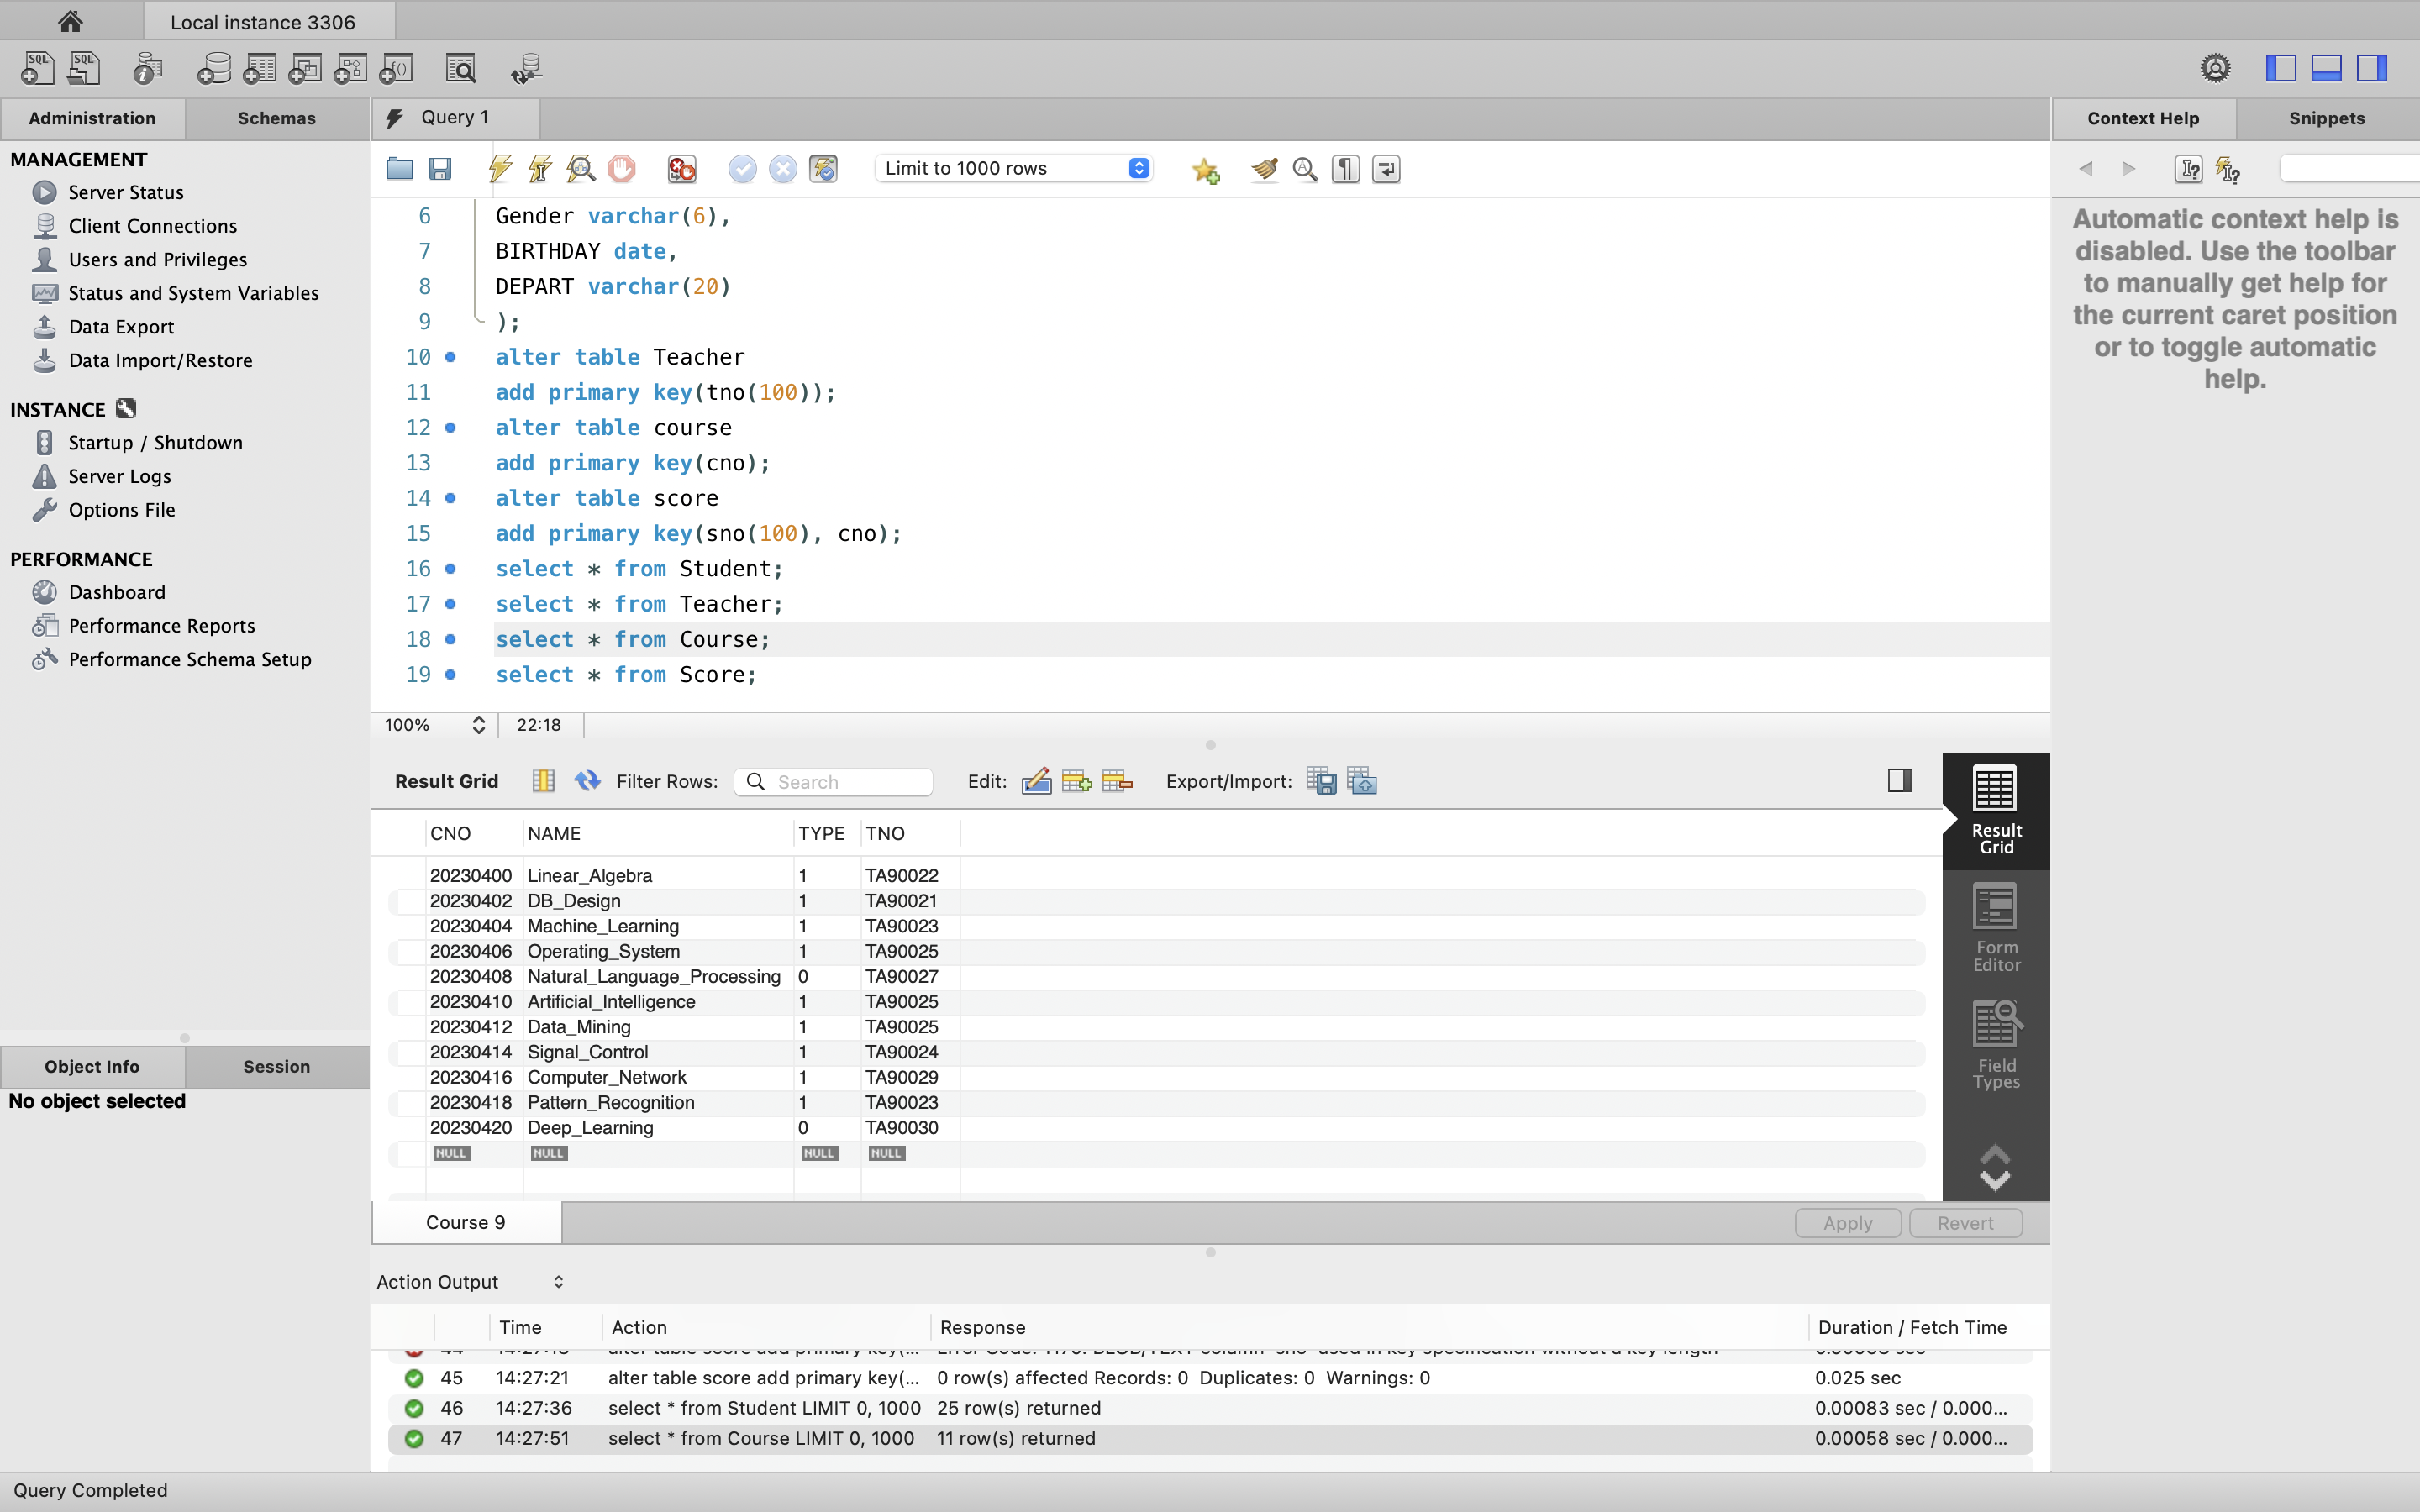
\includegraphics[scale=0.1]{pics/Course.png}
  \caption*{Course}
\end{figure}
\begin{figure}[H]
  \centering
  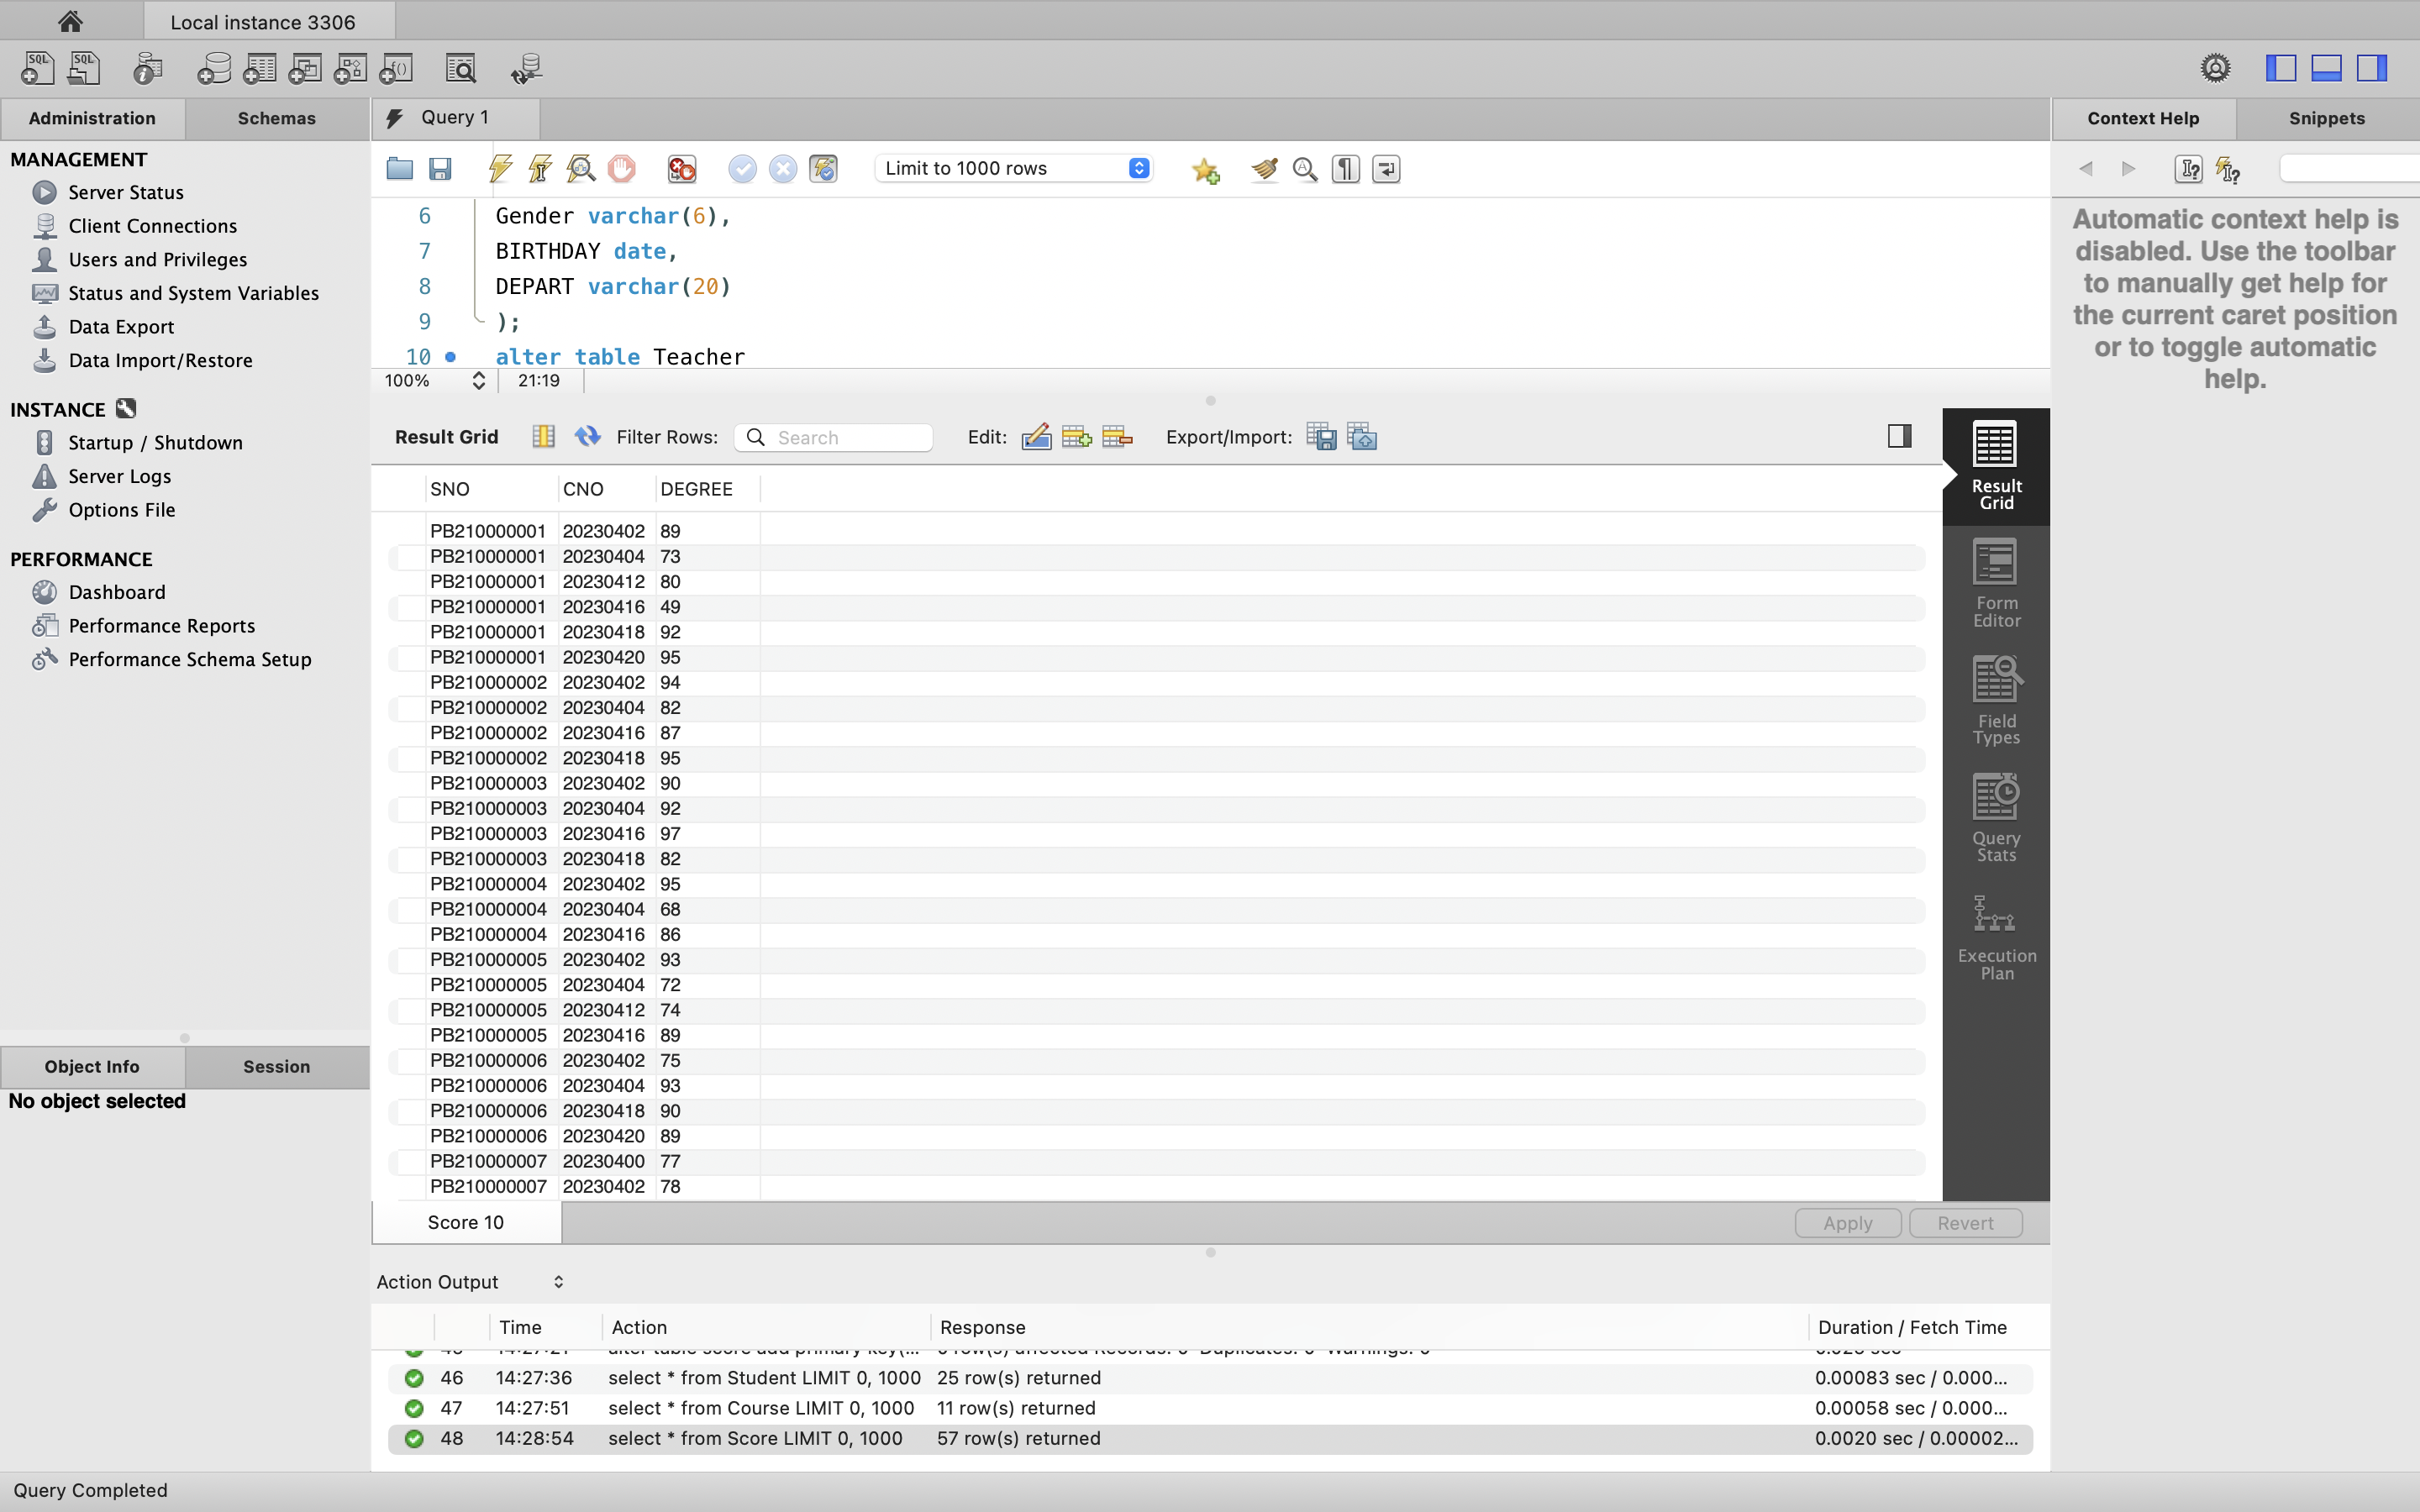
\includegraphics[scale=0.1]{pics/Score.png}
  \caption*{Score}
\end{figure}
\begin{figure}[H]
  \centering
  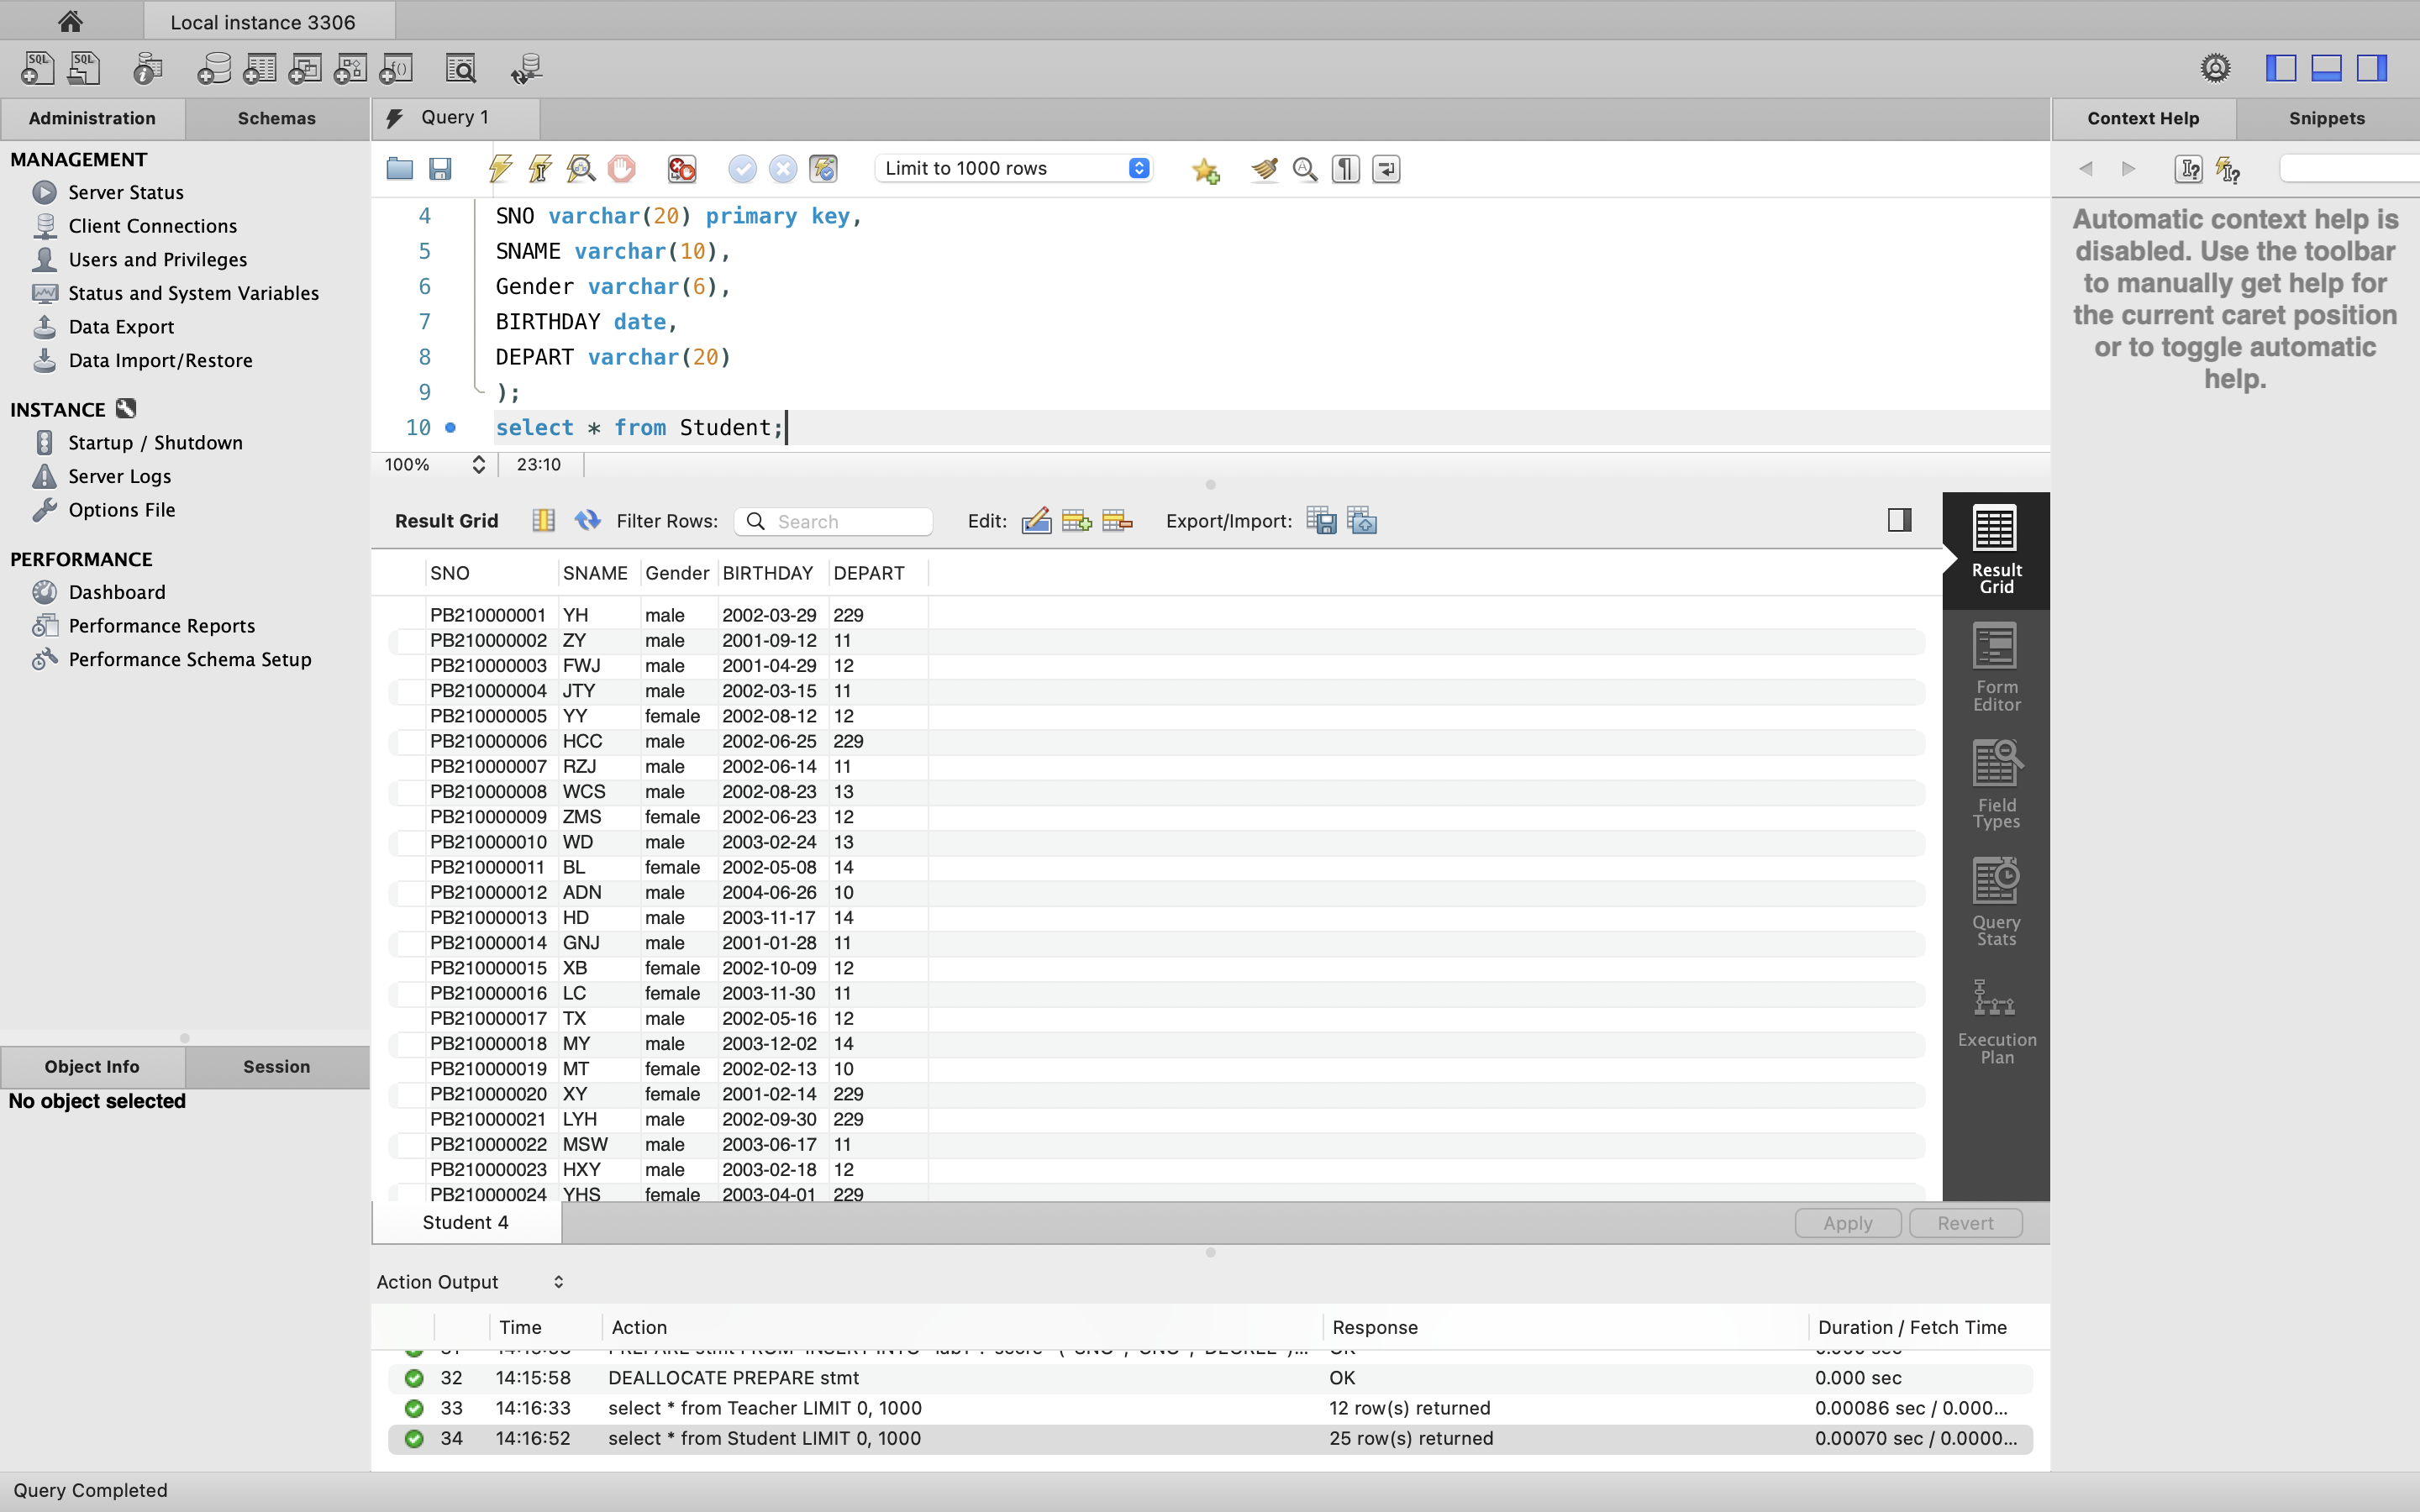
\includegraphics[scale=0.1]{pics/Student.png}
  \caption*{Student}
\end{figure}
\begin{figure}[H]
  \centering
  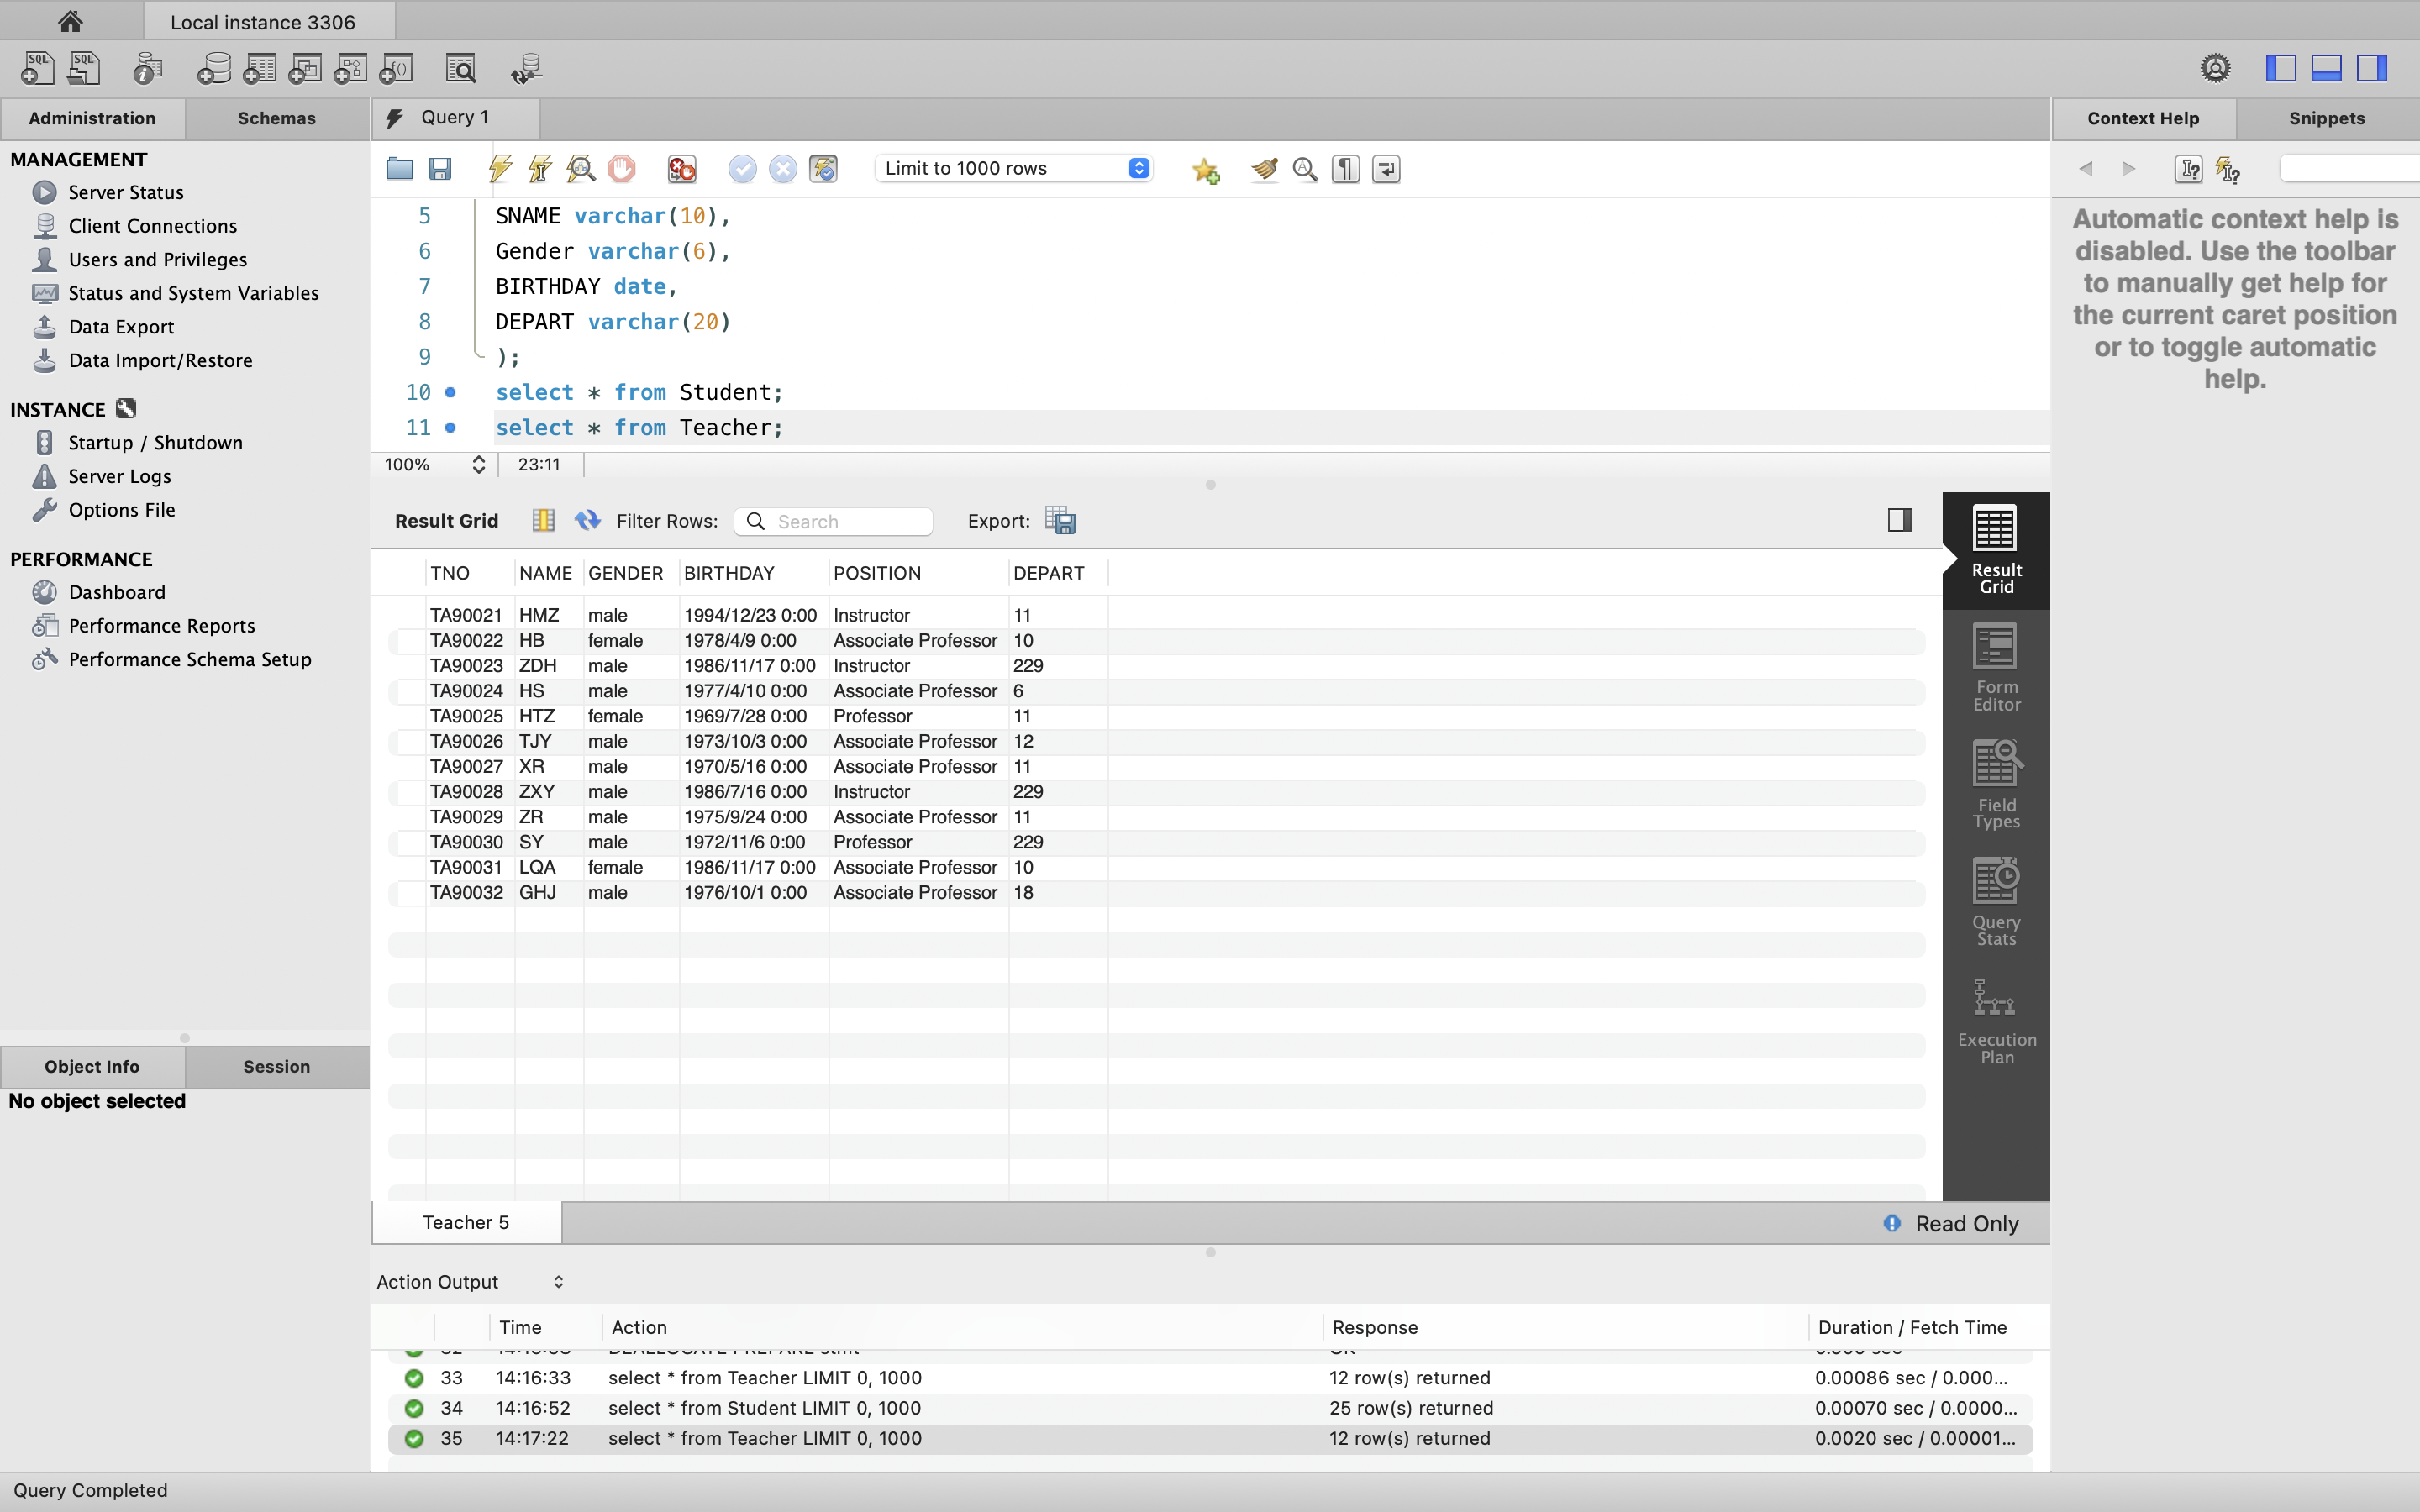
\includegraphics[scale=0.1]{pics/Teacher.png}
  \caption*{Teacher}
\end{figure}

\section{任务二}

\subsection{}
\begin{lstlisting}
  ALTER TABLE Student
  ADD COLUMN AGE INT;
\end{lstlisting}
\begin{figure}[H]
  \centering
  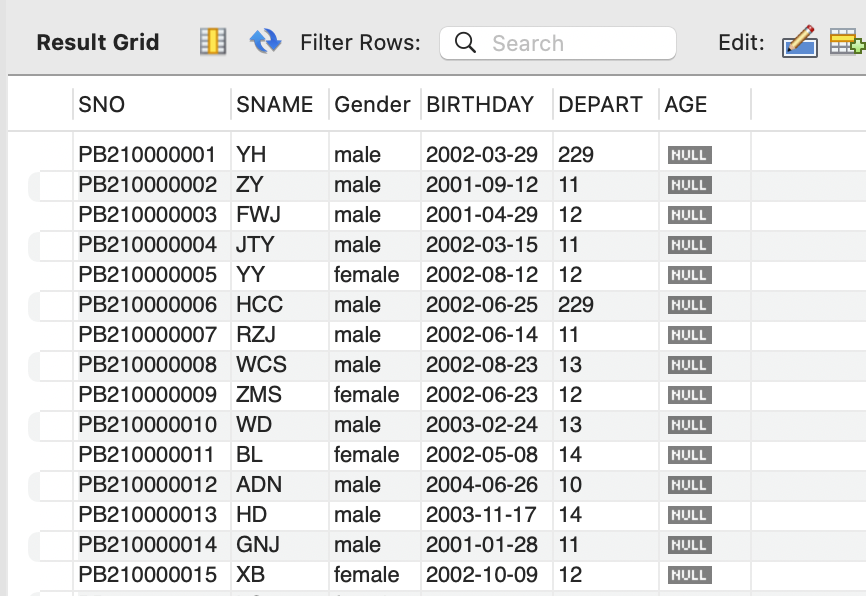
\includegraphics[scale=0.4]{pics/1.png}
  \caption*{T1}
\end{figure}

\subsection{}
\begin{lstlisting}
  UPDATE Student
  SET AGE = YEAR(CURDATE())-YEAR(BIRTHDAY);
\end{lstlisting}
\begin{figure}[H]
  \centering
  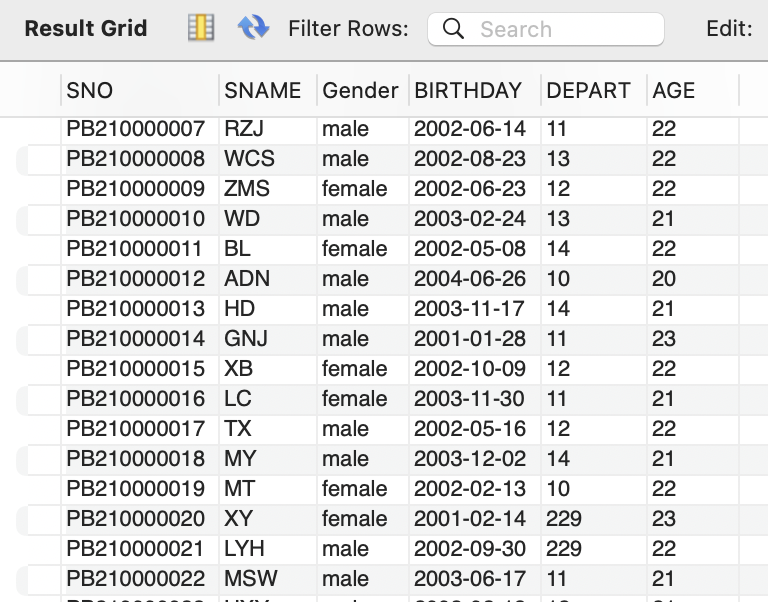
\includegraphics[scale=0.4]{pics/2.png}
  \caption*{T2}
\end{figure}

\subsection{}
\begin{lstlisting}
  UPDATE Student
  SET AGE = AGE + 2;
  ALTER TABLE Student
  MODIFY AGE CHAR(3);
\end{lstlisting}
\begin{figure}[H]
  \centering
  \begin{minipage}{0.4\linewidth}
    \includegraphics*[scale=0.4]{pics/3_1.png}
  \end{minipage}
  \begin{minipage}{0.4\linewidth}
    \includegraphics*[scale=0.3]{pics/3_2.png}
  \end{minipage}
  \caption*{T3}
\end{figure}

\subsection{}
\begin{lstlisting}
  ALTER TABLE Student
  DROP COLUMN AGE;
\end{lstlisting}
\begin{figure}[H]
  \centering
  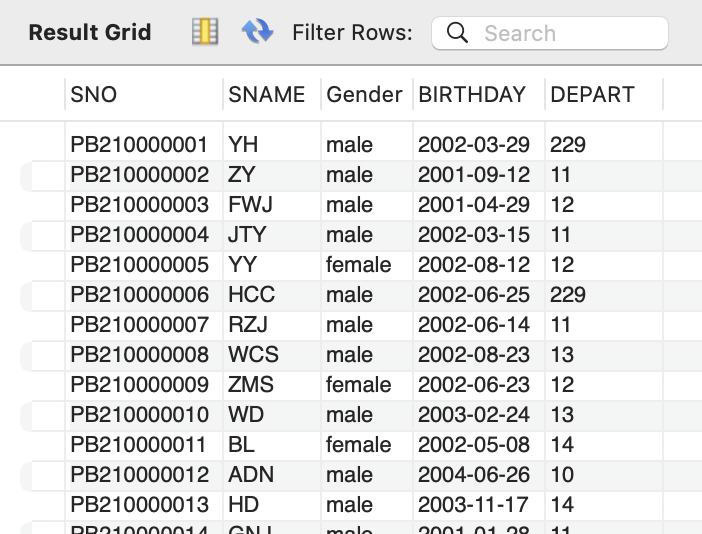
\includegraphics[scale=0.4]{pics/4.png}
  \caption*{T4}
\end{figure}

\subsection{}
\begin{lstlisting}
  CREATE TABLE teacher_course AS
  SELECT TNO
  FROM Teacher;
  ALTER TABLE teacher_course
    ADD PRIMARY KEY (TNO(20)),
    ADD COLUMN NUM_COURSE INT;
\end{lstlisting}
\begin{figure}[H]
  \centering
  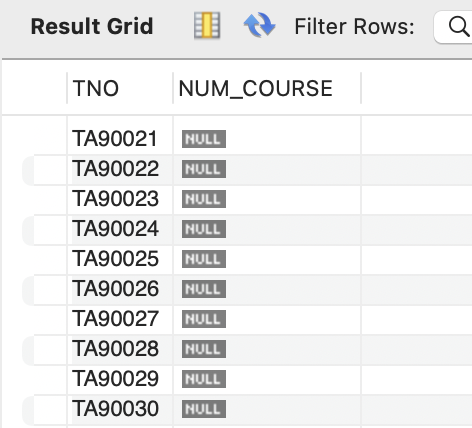
\includegraphics[scale=0.5]{pics/5.png}
  \caption*{T5}
\end{figure}

\subsection{}
\begin{lstlisting}
  UPDATE teacher_course tc
  LEFT JOIN (
      SELECT TNO, COUNT(*) as num_courses
      FROM course
      GROUP BY TNO
  ) c ON tc.TNO = c.TNO
  SET tc.NUM_COURSE = c.num_courses;
\end{lstlisting}
\begin{figure}[H]
  \centering
  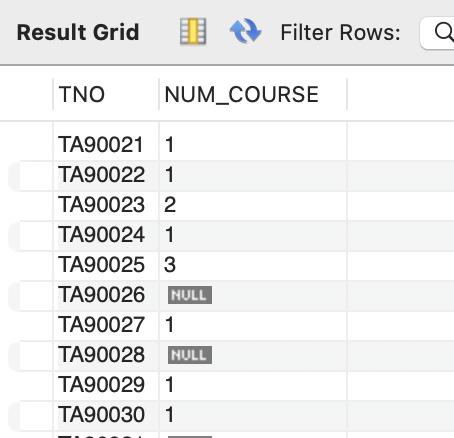
\includegraphics[scale=0.5]{pics/6.png}
  \caption*{T6}
\end{figure}

\subsection{}
\begin{lstlisting}
  DELETE FROM teacher_course
  WHERE NUM_COURSE IS NULL;
\end{lstlisting}
\begin{figure}[H]
  \centering
  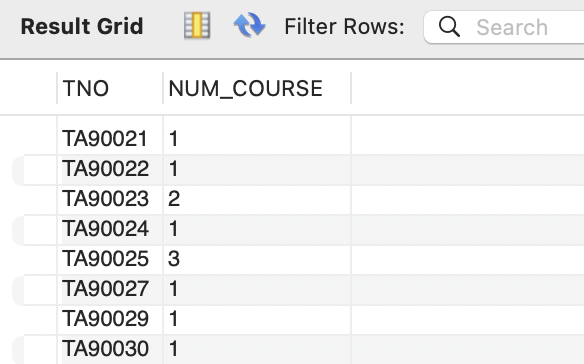
\includegraphics[scale=0.5]{pics/7.png}
  \caption*{T7}
\end{figure}

\subsection{}
\begin{lstlisting}
  DROP TABLE teacher_course;
\end{lstlisting}
\begin{figure}[H]
  \centering
  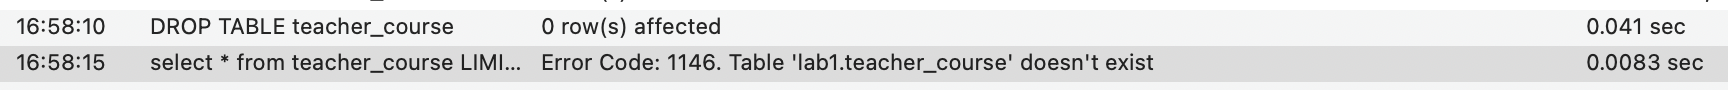
\includegraphics[scale=0.4]{pics/8.png}
  \caption*{T8}
\end{figure}

\subsection{}
\begin{lstlisting}
  INSERT INTO Student(SNO, SNAME, Gender, BIRTHDAY, DEPART)
  VALUES	('PB22151743', 'CSQ', 'male', '2005-02-04', '229'),
      ('PB22114514', 'ABC', 'male', '2004-08-10', '15'),
      ('PB21919810', 'DEF', 'female', '2004-03-16', '11');
  INSERT INTO Score(SNO, CNO, DEGREE)
  VALUES	('PB22151743', 20230402, 98),
      ('PB22151743', 20230410, 99),
      ('PB22151743', 20230412, 97);
\end{lstlisting}
\begin{figure}[H]
  \centering
  \begin{minipage}{0.4\linewidth}
    \includegraphics*[scale=0.5]{pics/9_1.png}
  \end{minipage}
  \begin{minipage}{0.4\linewidth}
    \includegraphics*[scale=0.5]{pics/9_2.png}
  \end{minipage}
  \caption*{T9}
\end{figure}

\subsection{}
\begin{lstlisting}
  DELETE s FROM score s
  JOIN (
      SELECT MIN(DEGREE) as min_degree
      FROM score
      WHERE SNO = 'PB22151743'
  ) as t
  ON s.DEGREE = t.min_degree
  WHERE s.SNO = 'PB22151743';
\end{lstlisting}
\begin{figure}[H]
  \centering
  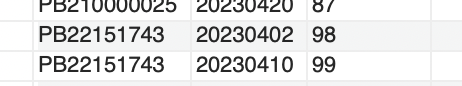
\includegraphics[scale=0.7]{pics/10.png}
  \caption*{T10}
\end{figure}

\subsection{}
\begin{lstlisting}
  CREATE INDEX NAME_INDEX ON Course(NAME(20));
\end{lstlisting}
\begin{figure}[H]
  \centering
  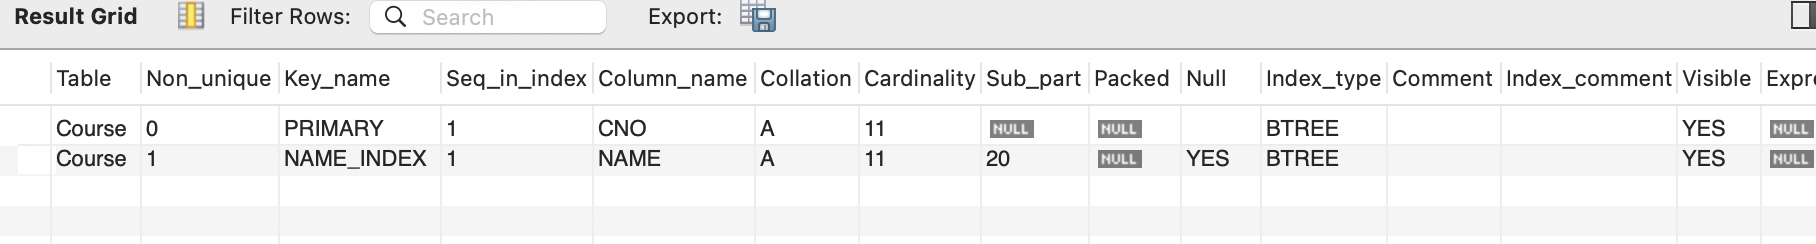
\includegraphics[scale=0.4]{pics/11.png}
  \caption*{T11}
\end{figure}

\subsection{}
\begin{lstlisting}
  CREATE UNIQUE INDEX TNO_INDEX ON Teacher(TNO(10));
\end{lstlisting}
\begin{figure}[H]
  \centering
  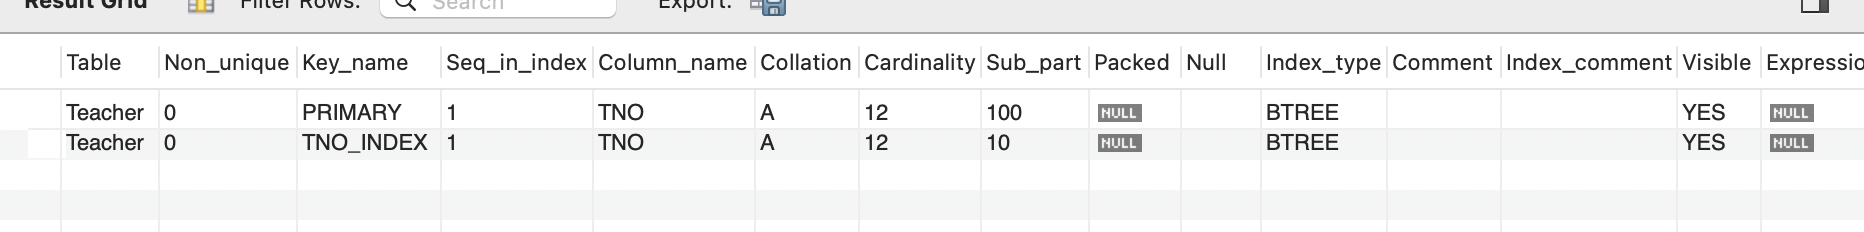
\includegraphics[scale=0.4]{pics/12.png}
  \caption*{T12}
\end{figure}

\subsection{}
\begin{lstlisting}
  CREATE INDEX RECORD_INDEX ON Score (SNO(20) DESC, DEGREE ASC);
\end{lstlisting}
\begin{figure}[H]
  \centering
  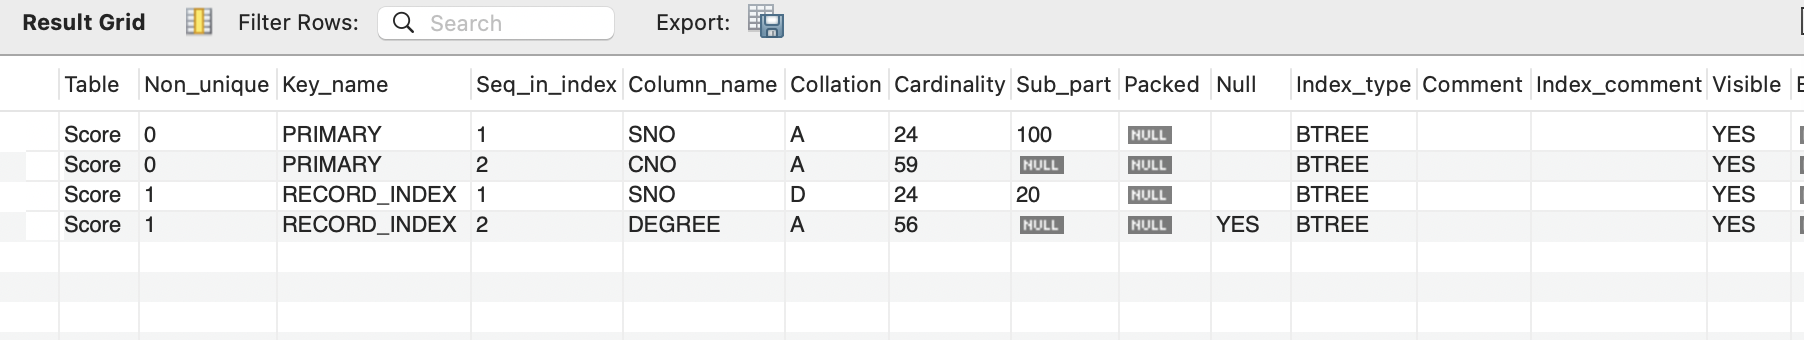
\includegraphics[scale=0.4]{pics/13.png}
  \caption*{T13}
\end{figure}

\subsection{}
\begin{lstlisting}
  SHOW INDEX FROM score;
\end{lstlisting}
\begin{figure}[H]
  \centering
  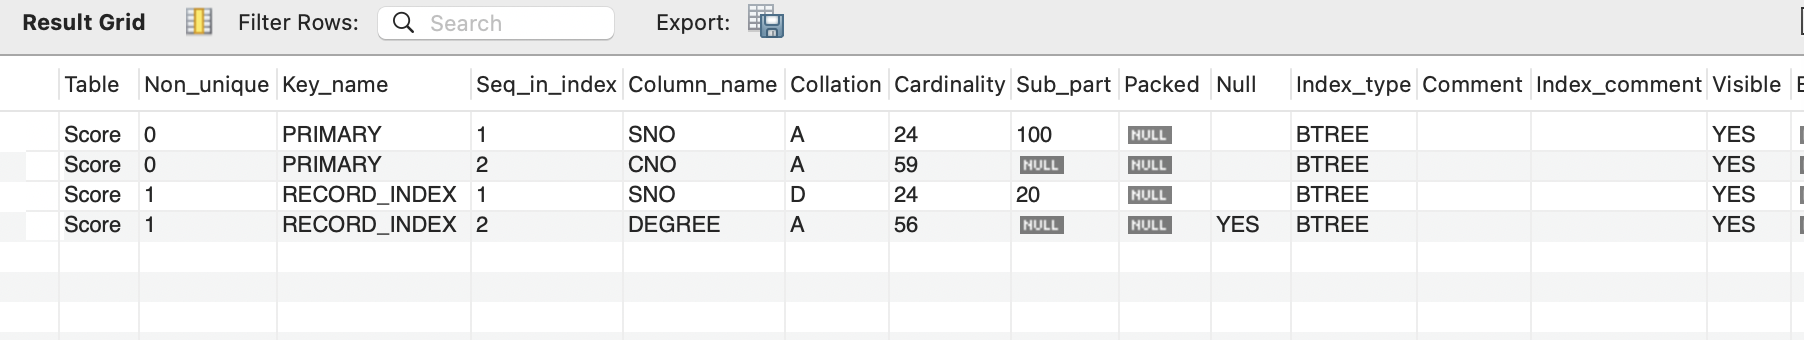
\includegraphics[scale=0.4]{pics/13.png}
  \caption*{T14}
\end{figure}

\subsection{}
\begin{lstlisting}
  ALTER TABLE Teacher DROP INDEX TNO_INDEX;
\end{lstlisting}
\begin{figure}[H]
  \centering
  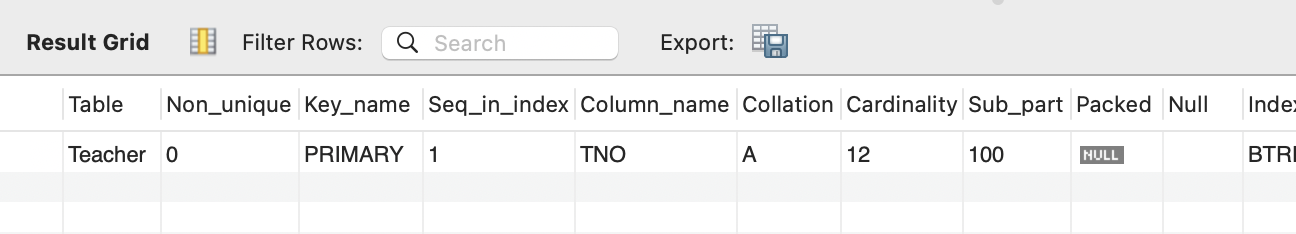
\includegraphics[scale=0.4]{pics/15.png}
  \caption*{T15}
\end{figure}

\subsection{}
\begin{lstlisting}
  SELECT SNO, SNAME
  FROM Student
  WHERE DEPART = (
      SELECT DEPART
      FROM Student
      WHERE SNO = 'your_student_number'
  );  
\end{lstlisting}
\begin{figure}[H]
  \centering
  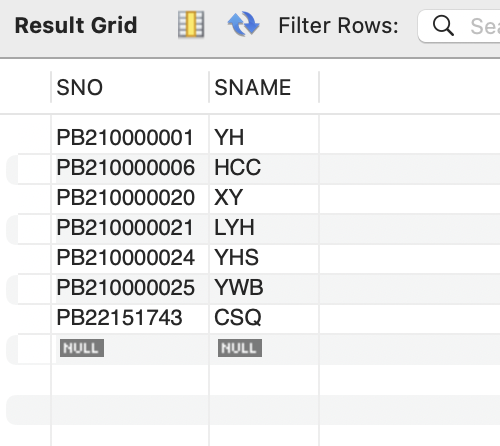
\includegraphics[scale=0.7]{pics/16.png}
  \caption*{T16}
\end{figure}

\subsection{}
\begin{lstlisting}
  SELECT SNO, SNAME
  FROM Student
  WHERE DEPART = (
      SELECT DEPART
      FROM Student
      WHERE SNO = 'PB22151743'
  ) AND SNO != 'PB22151743';
\end{lstlisting}
\begin{figure}[H]
  \centering
  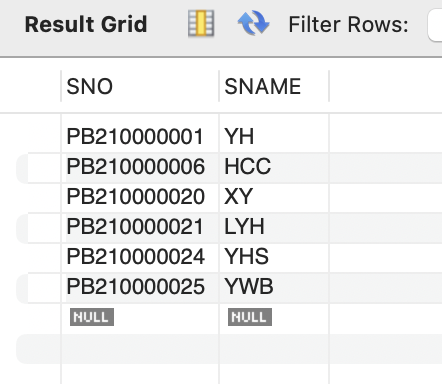
\includegraphics[scale=0.7]{pics/17.png}
  \caption*{T17}
\end{figure}

\subsection{}
\begin{lstlisting}
  SELECT SNO, SNAME
  FROM Student
  WHERE DEPART = (
      SELECT DEPART
      FROM Student
      WHERE SNO = 'PB22114514'
  );
\end{lstlisting}
\begin{figure}[H]
  \centering
  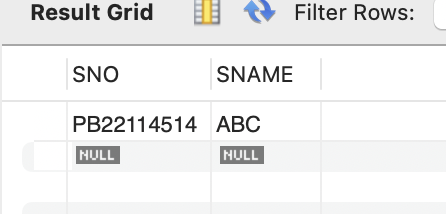
\includegraphics[scale=0.7]{pics/18.png}
  \caption*{T18}
\end{figure}

\subsection{}
\begin{lstlisting}
  SELECT SNO, SNAME
  FROM Student
  WHERE DEPART NOT IN (
      SELECT DEPART
      FROM Student
      WHERE SNO IN ('PB22114514', 'PB21919810')
  );
\end{lstlisting}
\begin{figure}[H]
  \centering
  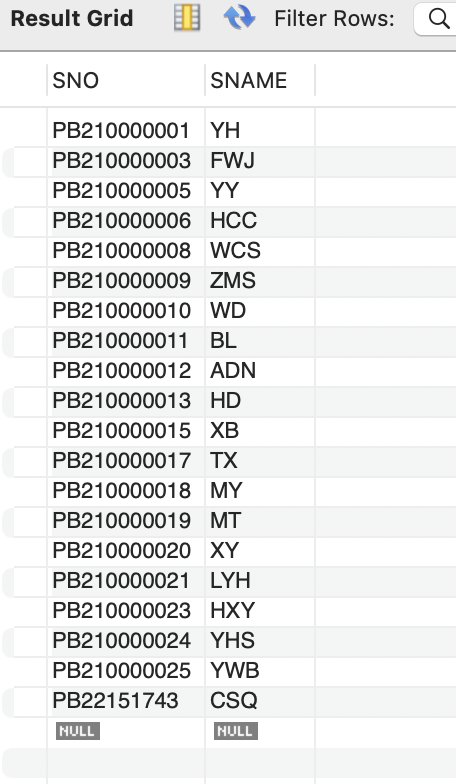
\includegraphics[scale=0.7]{pics/19.png}
  \caption*{T19}
\end{figure}

\subsection{}
\begin{lstlisting}
  SELECT TNO, TNAME
  FROM Teacher
  WHERE TNO IN(
    SELECT TNO
      FROM Course
      WHERE CNO IN(
      SELECT CNO
          FROM Score
          WHERE SNO = ("PB22151743")
    )
  );
\end{lstlisting}
\begin{figure}[H]
  \centering
  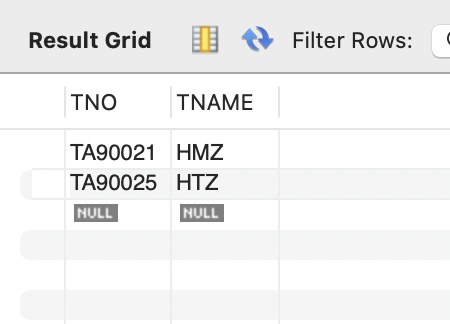
\includegraphics[scale=0.7]{pics/20.png}
  \caption*{T20}
\end{figure}

\subsection{}
\begin{lstlisting}
  SELECT COUNT(*)
  FROM Teacher
  WHERE DEPART IN ('11', '229');
\end{lstlisting}
\begin{figure}[H]
  \centering
  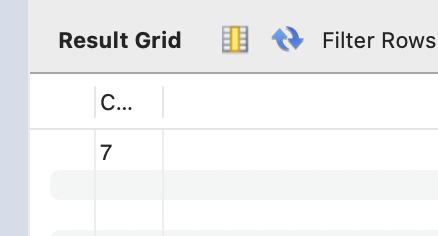
\includegraphics[scale=0.7]{pics/21.png}
  \caption*{T21}
\end{figure}

\subsection{}
\begin{lstlisting}
  SELECT SNO, SNAME, YEAR(CURDATE()) - YEAR(BIRTHDAY) AS Age
  FROM Student
  WHERE DEPART = (
      SELECT DEPART
      FROM Student
      WHERE SNO = 'PB22151743'
  );
\end{lstlisting}
\begin{figure}[H]
  \centering
  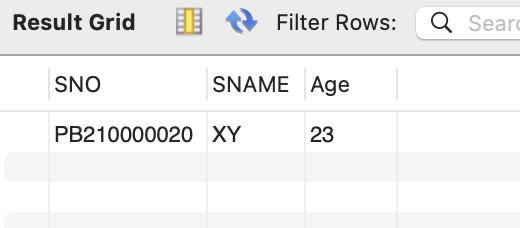
\includegraphics[scale=0.7]{pics/22.png}
  \caption*{T22}
\end{figure}

\subsection{}
\begin{lstlisting}
  SELECT SNO, SNAME, YEAR(CURDATE()) - YEAR(BIRTHDAY) AS Age
  FROM Student
  WHERE DEPART = (
      SELECT DEPART
      FROM Student
      WHERE SNO = 'PB22151743'
  )
  ORDER BY Age ASC
  LIMIT 1;
\end{lstlisting}
\begin{figure}[H]
  \centering
  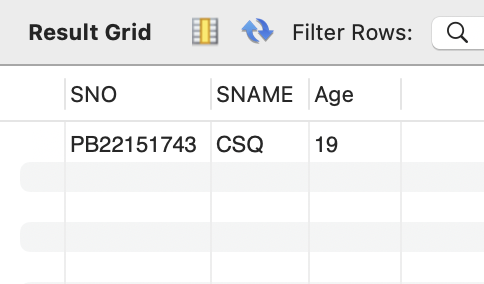
\includegraphics[scale=0.7]{pics/23.png}
  \caption*{T23}
\end{figure}

\subsection{}
\begin{lstlisting}
  SELECT s.SNO, s.SNAME, sc.DEGREE
  FROM Student s
  JOIN score sc ON s.SNO = sc.SNO
  JOIN Course c ON sc.CNO = c.CNO
  WHERE c.NAME = 'DB_Design' AND sc.DEGREE < 75;
\end{lstlisting}
\begin{figure}[H]
  \centering
  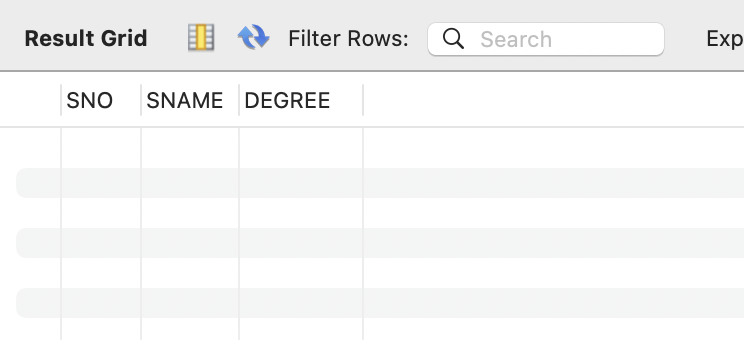
\includegraphics[scale=0.7]{pics/24.png}
  \caption*{T24}
\end{figure}

\subsection{}
\begin{lstlisting}
  SELECT DISTINCT s.SNO, s.SNAME
  FROM Student s
  JOIN score sc ON s.SNO = sc.SNO
  JOIN Course c ON sc.CNO = c.CNO
  JOIN Teacher t ON c.TNO = t.TNO
  WHERE t.TNAME = 'ZDH';
\end{lstlisting}
\begin{figure}[H]
  \centering
  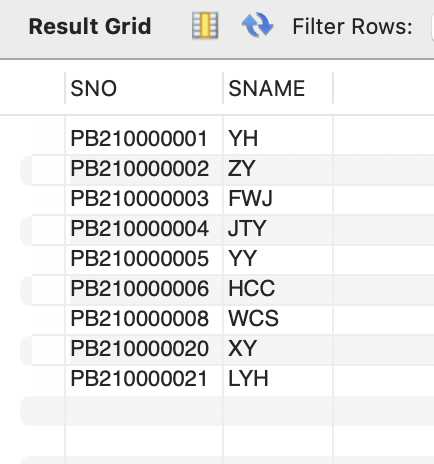
\includegraphics[scale=0.7]{pics/25.png}
  \caption*{T25}
\end{figure}

\subsection{}
\begin{lstlisting}
  SELECT sc.SNO, sc.DEGREE
  FROM score sc
  JOIN Course c ON sc.CNO = c.CNO
  WHERE c.NAME = 'Machine_Learning'
  ORDER BY sc.DEGREE DESC;
\end{lstlisting}
\begin{figure}[H]
  \centering
  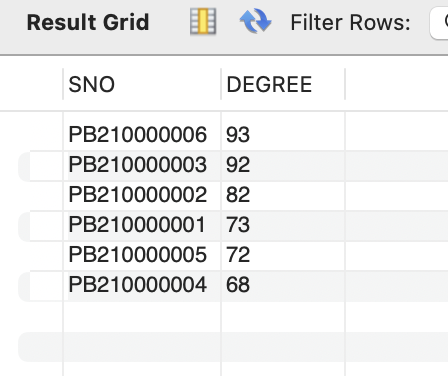
\includegraphics[scale=0.7]{pics/26.png}
  \caption*{T26}
\end{figure}

\subsection{}
\begin{lstlisting}
  SELECT c.CNO, c.NAME, AVG(sc.DEGREE) AS Average_Score
  FROM Course c
  LEFT JOIN score sc ON c.CNO = sc.CNO
  GROUP BY c.CNO, c.NAME;  
\end{lstlisting}
\begin{figure}[H]
  \centering
  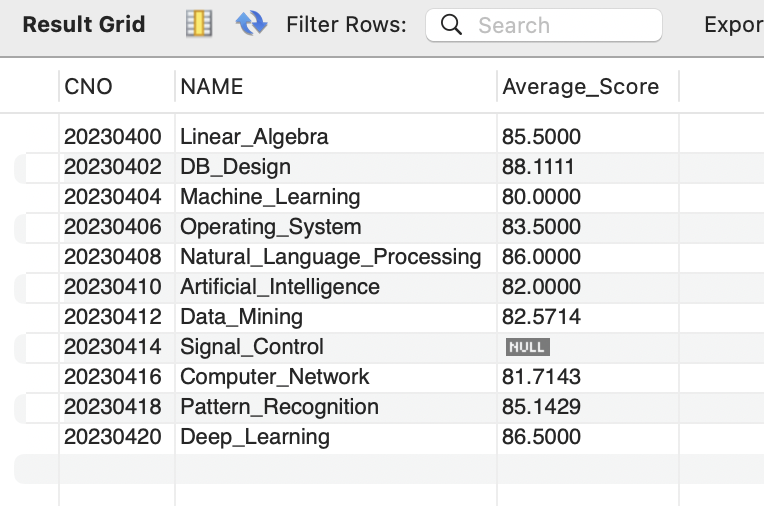
\includegraphics[scale=0.7]{pics/27.png}
  \caption*{T27}
\end{figure}

\subsection{}
\begin{lstlisting}
  SELECT c.CNO, c.NAME, AVG(sc.DEGREE) AS Average_Score
  FROM Course c
  LEFT JOIN score sc ON c.CNO = sc.CNO
  WHERE c.TYPE = 1
  GROUP BY c.CNO, c.NAME;  
\end{lstlisting}
\begin{figure}[H]
  \centering
  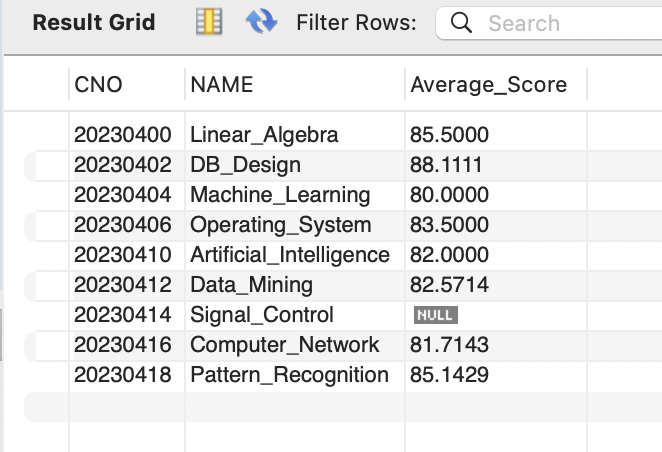
\includegraphics[scale=0.7]{pics/28.png}
  \caption*{T28}
\end{figure}

\subsection{}
\begin{lstlisting}
  SELECT s.SNO
  FROM Student s
  JOIN score sc ON s.SNO = sc.SNO
  JOIN Course c ON sc.CNO = c.CNO
  WHERE c.TNO = 'TA90023'
  GROUP BY s.SNO
  HAVING COUNT(DISTINCT c.CNO) = (SELECT COUNT(*) FROM Course WHERE TNO = 'TA90023');
\end{lstlisting}
\begin{figure}[H]
  \centering
  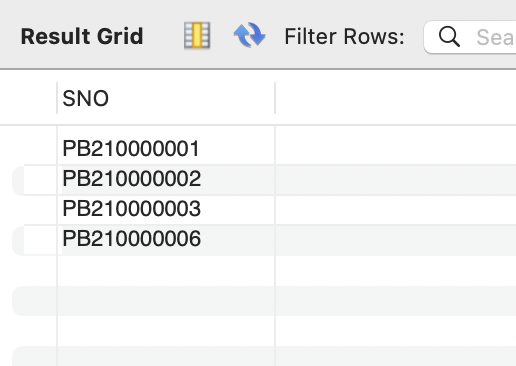
\includegraphics[scale=0.7]{pics/29.png}
  \caption*{T29}
\end{figure}

\subsection{}
\begin{lstlisting}
  SELECT c.CNO, c.NAME, MAX(sc.DEGREE) AS Max_Score, MIN(sc.DEGREE) AS Min_Score, MAX(sc.DEGREE) - MIN(sc.DEGREE) AS Score_Difference
  FROM Course c
  JOIN score sc ON c.CNO = sc.CNO
  GROUP BY c.CNO, c.NAME;  
\end{lstlisting}
\begin{figure}[H]
  \centering
  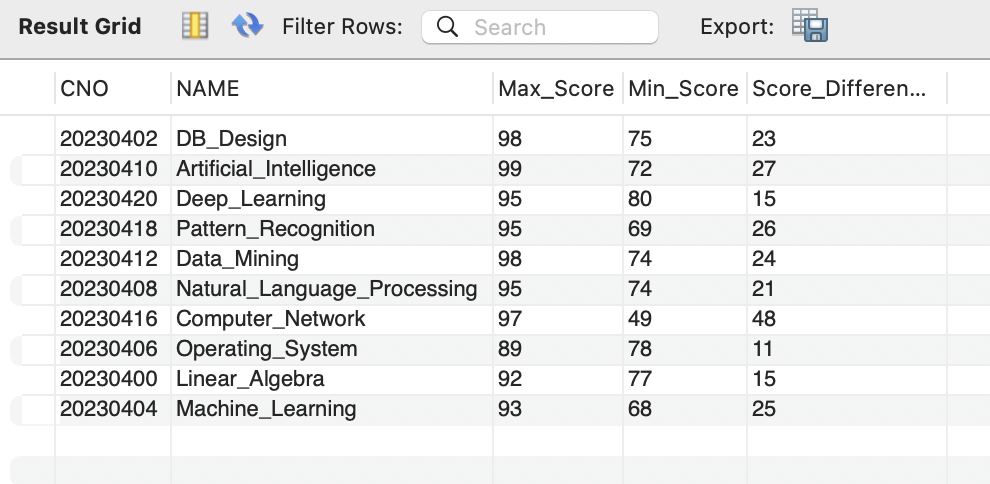
\includegraphics[scale=0.7]{pics/30.png}
  \caption*{T30}
\end{figure}

\subsection{}
\begin{lstlisting}
  SELECT sc.SNO, COUNT(sc.CNO) AS Courses_Below_75
  FROM score sc
  WHERE sc.DEGREE < 75
  GROUP BY sc.SNO;  
\end{lstlisting}
\begin{figure}[H]
  \centering
  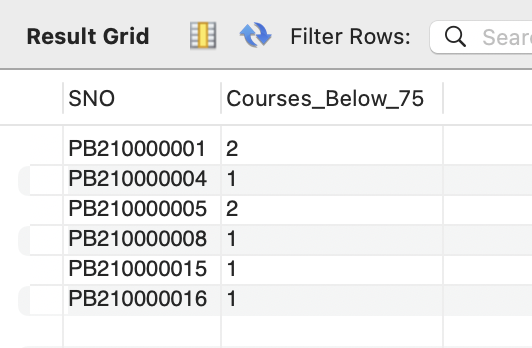
\includegraphics[scale=0.7]{pics/31.png}
  \caption*{T31}
\end{figure}

\subsection{}
\begin{lstlisting}
  SELECT DISTINCT t.TNO, t.TNAME
  FROM Teacher t
  JOIN Course c ON t.TNO = c.TNO
  JOIN score sc ON c.CNO = sc.CNO
  WHERE sc.DEGREE < 75;  
\end{lstlisting}
\begin{figure}[H]
  \centering
  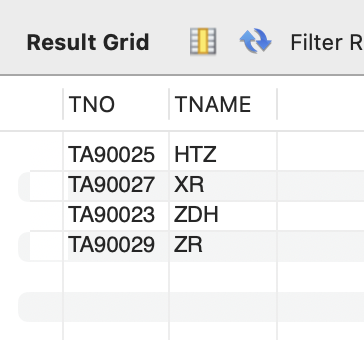
\includegraphics[scale=0.7]{pics/32.png}
  \caption*{T32}
\end{figure}

\subsection{}
\begin{lstlisting}
  SELECT s.SNO, s.SNAME
  FROM Student s
  JOIN score sc ON s.SNO = sc.SNO
  GROUP BY s.SNO, s.SNAME
  HAVING COUNT(DISTINCT sc.CNO) < 2;  
\end{lstlisting}
\begin{figure}[H]
  \centering
  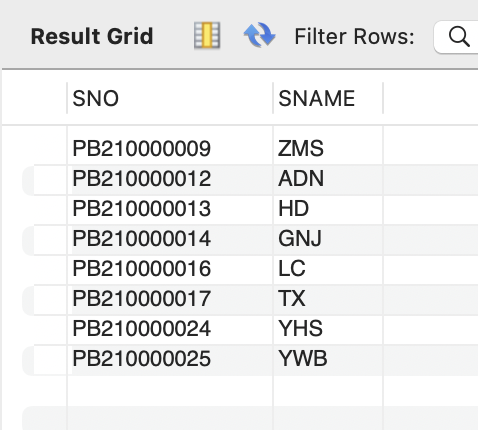
\includegraphics[scale=0.7]{pics/33.png}
  \caption*{T33}
\end{figure}

\subsection{}
\begin{lstlisting}
  SELECT sc.SNO
  FROM score sc
  WHERE NOT EXISTS (
      SELECT c.CNO
      FROM score c
      WHERE c.SNO = 'PB210000001'
      AND c.CNO NOT IN (
          SELECT sc2.CNO
          FROM score sc2
          WHERE sc2.SNO = sc.SNO
      )
  )
  GROUP BY sc.SNO
  HAVING COUNT(DISTINCT sc.CNO) >= (
      SELECT COUNT(DISTINCT c.CNO)
      FROM score c
      WHERE c.SNO = 'PB210000001'
  );   
\end{lstlisting}
\begin{figure}[H]
  \centering
  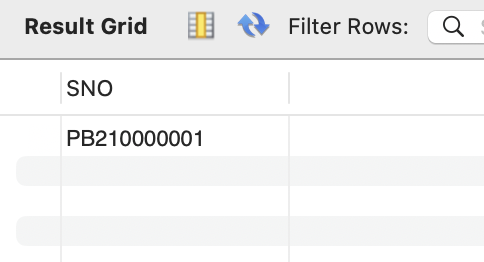
\includegraphics[scale=0.7]{pics/34.png}
  \caption*{T34}
\end{figure}

\subsection{}
\begin{lstlisting}
  SELECT c.NAME, AVG(sc.DEGREE) AS Average_Score
  FROM Course c
  LEFT JOIN score sc ON c.CNO = sc.CNO
  GROUP BY c.NAME;  
\end{lstlisting}
\begin{figure}[H]
  \centering
  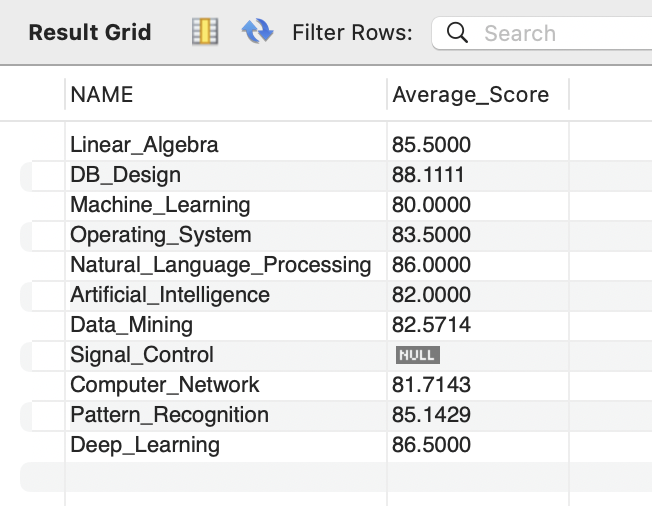
\includegraphics[scale=0.7]{pics/35.png}
  \caption*{T35}
\end{figure}

\subsection{}
\begin{lstlisting}
  SELECT s.DEPART, COUNT(DISTINCT s.SNO) AS Total_Students, AVG(sc.DEGREE) AS Average_Score
  FROM Student s
  LEFT JOIN score sc ON s.SNO = sc.SNO
  GROUP BY s.DEPART;  
\end{lstlisting}
\begin{figure}[H]
  \centering
  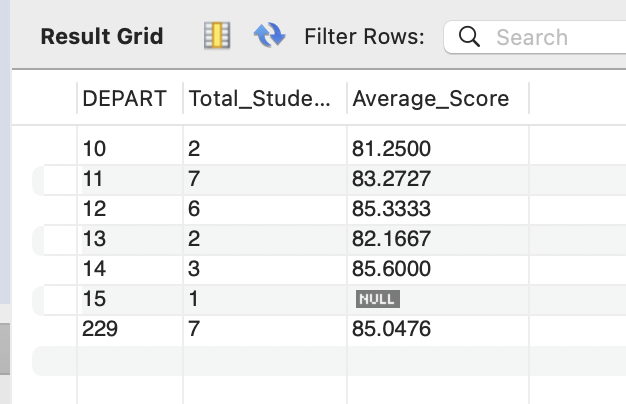
\includegraphics[scale=0.7]{pics/36.png}
  \caption*{T36}
\end{figure}

\subsection{}
\begin{lstlisting}
  SELECT DISTINCT s.SNAME
  FROM Student s
  WHERE s.SNO NOT IN (
      SELECT sc.SNO
      FROM score sc
      JOIN Course c ON sc.CNO = c.CNO
      WHERE c.NAME IN ('DB_Design', 'Data_Mining')
  );  
\end{lstlisting}
\begin{figure}[H]
  \centering
  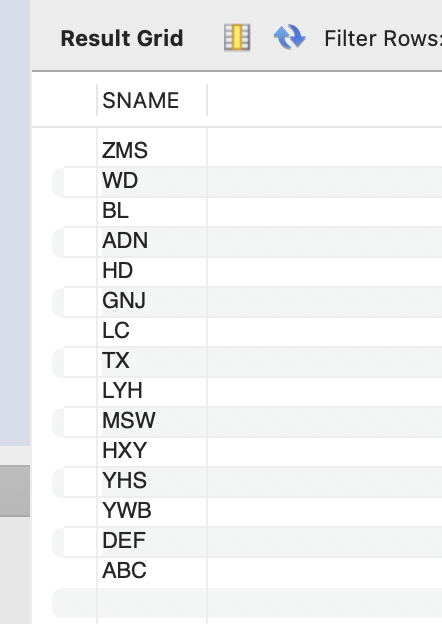
\includegraphics[scale=0.7]{pics/37.png}
  \caption*{T37}
\end{figure}

\subsection{}
\begin{lstlisting}
  SELECT c.NAME, MIN(YEAR(CURDATE()) - YEAR(s.BIRTHDAY)) AS Min_Age, 
  MAX(YEAR(CURDATE()) - YEAR(s.BIRTHDAY)) AS Max_Age, 
  AVG(YEAR(CURDATE()) - YEAR(s.BIRTHDAY)) AS Avg_Age
  FROM Course c
  LEFT JOIN score sc ON c.CNO = sc.CNO
  LEFT JOIN Student s ON sc.SNO = s.SNO
  GROUP BY c.NAME;
\end{lstlisting}
\begin{figure}[H]
  \centering
  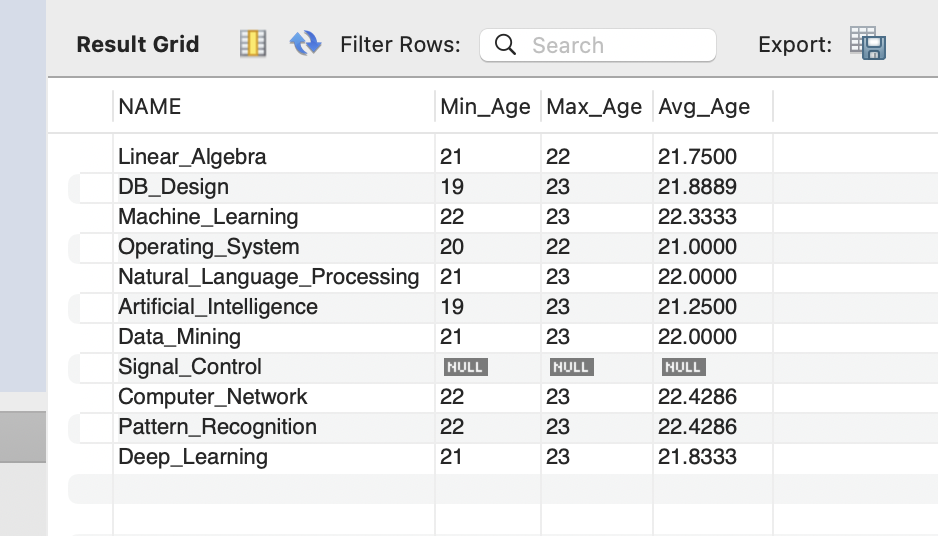
\includegraphics[scale=0.7]{pics/38.png}
  \caption*{T38}
\end{figure}

\subsection{}
\begin{lstlisting}
  SELECT DISTINCT s.SNO, s.SNAME
  FROM Student s
  JOIN score sc ON s.SNO = sc.SNO
  JOIN Course c ON sc.CNO = c.CNO
  WHERE c.NAME LIKE '%Computer%';  
\end{lstlisting}
\begin{figure}[H]
  \centering
  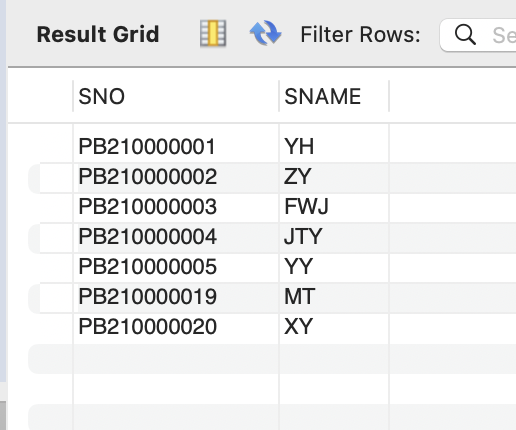
\includegraphics[scale=0.7]{pics/39.png}
  \caption*{T39}
\end{figure}

\subsection{}
\begin{lstlisting}
  SELECT sc.SNO, sc.CNO, sc.DEGREE
  FROM score sc
  JOIN (
      SELECT c.CNO, AVG(sc.DEGREE) AS Avg_Degree
      FROM Course c
      JOIN score sc ON c.CNO = sc.CNO
      GROUP BY c.CNO
  ) AS avg_scores ON sc.CNO = avg_scores.CNO
  WHERE sc.DEGREE BETWEEN (avg_scores.Avg_Degree - 12) AND (avg_scores.Avg_Degree + 12);  
\end{lstlisting}
\begin{figure}[H]
  \centering
  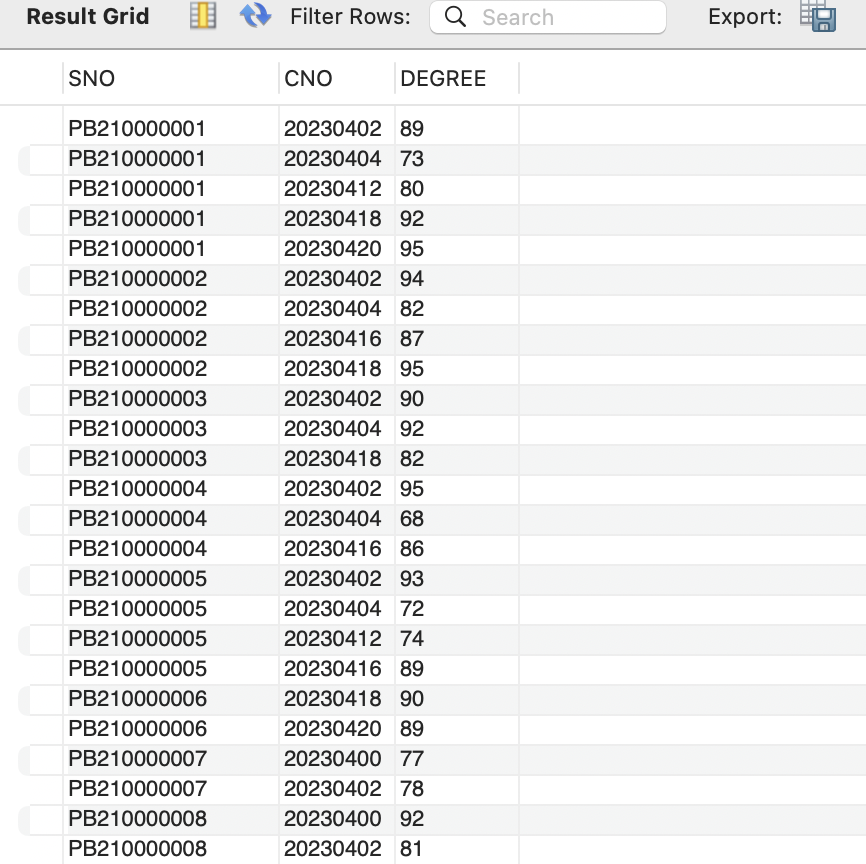
\includegraphics[scale=0.7]{pics/40.png}
  \caption*{T40}
\end{figure}

\subsection{}
\begin{lstlisting}
  CREATE VIEW db_229_student AS
  SELECT *
  FROM Student
  WHERE DEPART = '229'; 
\end{lstlisting}

\subsection{}
\begin{lstlisting}
  UPDATE db_229_student
  SET SNAME = 'J'
  WHERE SNO = 'PB210000020';  
\end{lstlisting}
\begin{figure}[H]
  \centering
  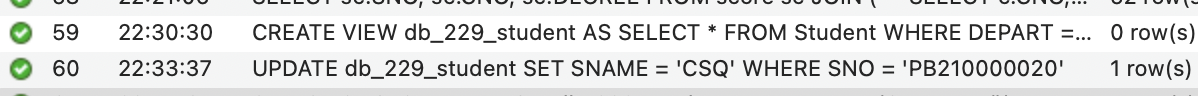
\includegraphics[scale=0.7]{pics/41-42.png}
  \caption*{T41\&42}
\end{figure}

\subsection{}
\begin{lstlisting}
  SELECT SNO, SNAME
  FROM db_229_student
  WHERE YEAR(CURDATE()) - YEAR(BIRTHDAY) < 22;
\end{lstlisting}
\begin{figure}[H]
  \centering
  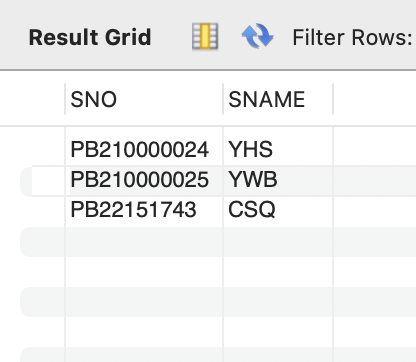
\includegraphics[scale=0.7]{pics/43.png}
  \caption*{T43}
\end{figure}

\subsection{}
\begin{lstlisting}
  INSERT INTO Student (SNO, SNAME, Gender, BIRTHDAY, DEPART)
  VALUES ('SA210110021', 'QXY', 'female', '2007-07-27', '229');
  SELECT * FROM db_229_student;
\end{lstlisting}
\begin{figure}[H]
  \centering
  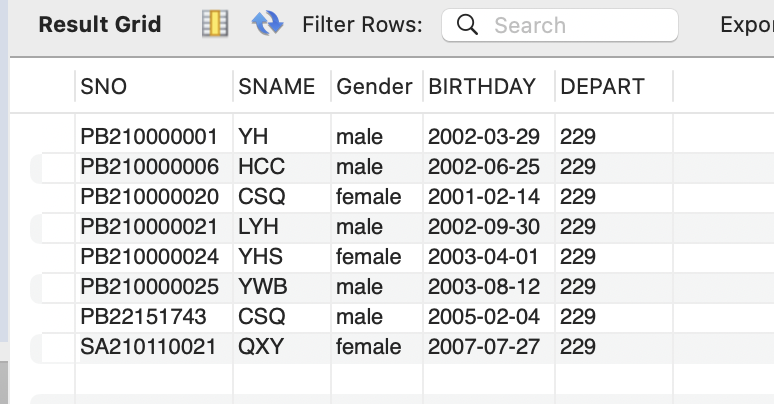
\includegraphics[scale=0.7]{pics/44.png}
  \caption*{T44}
\end{figure}

\subsection{}
\begin{lstlisting}
  INSERT INTO db_229_student (SNO, SNAME, Gender, BIRTHDAY, DEPART)
  VALUES ('SA210110023', 'DPC', 'male', '1997-04-27', '11');
\end{lstlisting}
\begin{figure}[H]
  \centering
  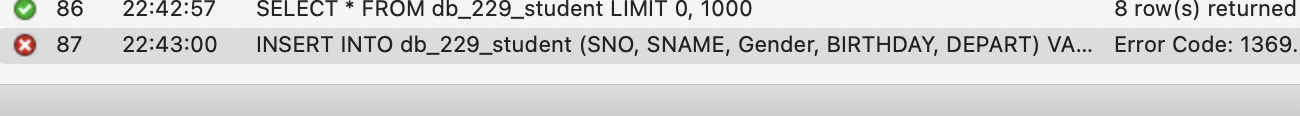
\includegraphics[scale=0.7]{pics/45.png}
  \caption*{T45}
\end{figure}
操作失败,不会影响视图内容,因为视图的定义限制了只能包含229系的学生。

\subsection{}
\begin{lstlisting}
  DROP VIEW db_229_student;
\end{lstlisting}
\begin{figure}[H]
  \centering
  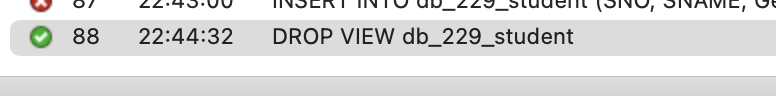
\includegraphics[scale=0.7]{pics/46.png}
  \caption*{T46}
\end{figure}

\subsection{}
\begin{lstlisting}
  CREATE TABLE teacher_salary (
    TNO VARCHAR(20),
    SAL FLOAT,
    PRIMARY KEY (TNO)
  );
\end{lstlisting}
\begin{figure}[H]
  \centering
  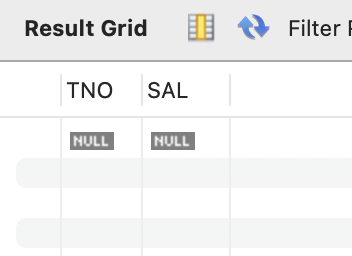
\includegraphics[scale=0.7]{pics/47.png}
  \caption*{T47}
\end{figure}

\subsection{}
\begin{lstlisting}
  DELIMITER $$
  CREATE TRIGGER check_teacher_existence_before_insert
  BEFORE INSERT ON teacher_salary
  FOR EACH ROW
  BEGIN
      IF NOT EXISTS (SELECT 1 FROM Teacher WHERE TNO = NEW.TNO) THEN
          SIGNAL SQLSTATE '45000'
          SET MESSAGE_TEXT = 'Error: TNO does not exist in the Teacher table.';
      END IF;
  END$$
  DELIMITER ;
  
  DELIMITER $$
  CREATE TRIGGER check_teacher_existence_before_update
  BEFORE UPDATE ON teacher_salary
  FOR EACH ROW
  BEGIN
      IF NOT EXISTS (SELECT 1 FROM Teacher WHERE TNO = NEW.TNO) THEN
          SIGNAL SQLSTATE '45000'
          SET MESSAGE_TEXT = 'Error: TNO does not exist in the Teacher table.';
      END IF;
  END$$
  DELIMITER ;
\end{lstlisting}
\begin{figure}[H]
  \centering
  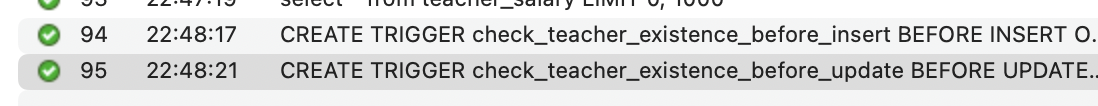
\includegraphics[scale=0.7]{pics/48.png}
  \caption*{T48}
\end{figure}

\subsection{}
\begin{lstlisting}
  DELIMITER $$
  CREATE TRIGGER salary_range_before_insert
  BEFORE INSERT ON teacher_salary
  FOR EACH ROW
  BEGIN
      DECLARE position VARCHAR(100);
      SELECT POSITION INTO position FROM Teacher WHERE TNO = NEW.TNO;
      CASE
          WHEN position = 'Instructor' THEN
              SET NEW.SAL = CASE
                  WHEN NEW.SAL < 4000 THEN 4000
                  WHEN NEW.SAL > 7000 THEN 7000
                  ELSE NEW.SAL
              END;
          WHEN position = 'Associate Professor' THEN
              SET NEW.SAL = CASE
                  WHEN NEW.SAL < 7000 THEN 7000
                  WHEN NEW.SAL > 10000 THEN 10000
                  ELSE NEW.SAL
              END;
          WHEN position = 'Professor' THEN
              SET NEW.SAL = CASE
                  WHEN NEW.SAL < 10000 THEN 10000
                  WHEN NEW.SAL > 13000 THEN 13000
                  ELSE NEW.SAL
              END;
      END CASE;
  END$$
  DELIMITER ;
  
  DELIMITER $$
  CREATE TRIGGER salary_range_before_update
  BEFORE UPDATE ON teacher_salary
  FOR EACH ROW
  BEGIN
      DECLARE position VARCHAR(100);
      SELECT POSITION INTO position FROM Teacher WHERE TNO = NEW.TNO;
      CASE
          WHEN position = 'Instructor' THEN
              SET NEW.SAL = CASE
                  WHEN NEW.SAL < 4000 THEN 4000
                  WHEN NEW.SAL > 7000 THEN 7000
                  ELSE NEW.SAL
              END;
          WHEN position = 'Associate Professor' THEN
              SET NEW.SAL = CASE
                  WHEN NEW.SAL < 7000 THEN 7000
                  WHEN NEW.SAL > 10000 THEN 10000
                  ELSE NEW.SAL
              END;
          WHEN position = 'Professor' THEN
              SET NEW.SAL = CASE
                  WHEN NEW.SAL < 10000 THEN 10000
                  WHEN NEW.SAL > 13000 THEN 13000
                  ELSE NEW.SAL
              END;
      END CASE;
  END$$
  DELIMITER ;
\end{lstlisting}
\begin{figure}[H]
  \centering
  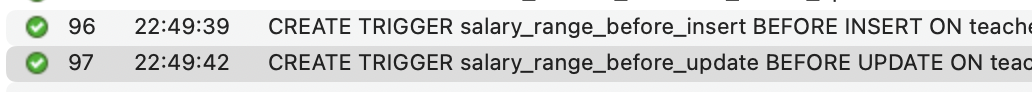
\includegraphics[scale=0.7]{pics/49.png}
  \caption*{T49}
\end{figure}

\subsection{}
\begin{lstlisting}
  DROP TRIGGER IF EXISTS check_teacher_existence_before_insert;
  DROP TRIGGER IF EXISTS check_teacher_existence_before_update;
  DROP TRIGGER IF EXISTS salary_range_before_insert;
  DROP TRIGGER IF EXISTS salary_range_before_update;
\end{lstlisting}
\begin{figure}[H]
  \centering
  \includegraphics[scale=0.7]{pics/50.png}
  \caption*{T50}
\end{figure}

\subsection{}
\begin{lstlisting}
  UPDATE score
  SET DEGREE = NULL
  WHERE CNO = (SELECT CNO FROM Course WHERE NAME = 'Data_Mining');
  SELECT SNO, DEGREE
  FROM score
  ORDER BY DEGREE ASC;
\end{lstlisting}
\begin{figure}[H]
  \centering
  \includegraphics[scale=0.7]{pics/51.png}
  \caption*{T51}
\end{figure}
可以看到,\lstinline|NULL|在升序排序中位于起始,推测其大小为0.

\subsection{}
查询选修了最多课程的学生.
\begin{lstlisting}
  SELECT s.SNO, s.SNAME, COUNT(sc.CNO) AS Courses_Count
  FROM Student s
  JOIN score sc ON s.SNO = sc.SNO
  GROUP BY s.SNO, s.SNAME
  ORDER BY Courses_Count DESC
  LIMIT 1;  
\end{lstlisting}
\begin{figure}[H]
  \centering
  \includegraphics[scale=0.7]{pics/52.png}
  \caption*{T52}
\end{figure}

\subsection{}
查询所教课堂中学生总数最多的教师.
\begin{lstlisting}
  SELECT t.TNO, t.TNAME, COUNT(DISTINCT sc.SNO) AS Total_Students
  FROM Teacher t
  JOIN Course c ON t.TNO = c.TNO
  JOIN score sc ON c.CNO = sc.CNO
  GROUP BY t.TNO, t.TNAME
  ORDER BY Total_Students DESC
  LIMIT 1;
\end{lstlisting}
\begin{figure}[H]
  \centering
  \includegraphics[scale=0.7]{pics/53.png}
  \caption*{T53}
\end{figure}

\bibliography{math}

\end{document}
\iffalse
\begin{figure}[h]
    \centering
    \includegraphics[scale=0.5]{name.png}
    \caption{name}
\end{figure}

\subsection{}
\begin{lstlisting}

\end{lstlisting}
\begin{figure}[H]
  \centering
  \includegraphics[scale=0.5]{pics/.png}
  \caption*{T}
\end{figure}
\fi

\lstset{
    language=Python,
    basicstyle=\small\ttfamily,
    keywordstyle=\color{blue},
    commentstyle=\color{green},
    stringstyle=\color{red},
    showstringspaces=false,
    breaklines=true,
}